\documentclass{article}
\usepackage{iclr2027_conference,times}

%%%%% NEW MATH DEFINITIONS %%%%%

\usepackage{amsmath,amsfonts,bm}

% Mark sections of captions for referring to divisions of figures
\newcommand{\figleft}{{\em (Left)}}
\newcommand{\figcenter}{{\em (Center)}}
\newcommand{\figright}{{\em (Right)}}
\newcommand{\figtop}{{\em (Top)}}
\newcommand{\figbottom}{{\em (Bottom)}}
\newcommand{\captiona}{{\em (a)}}
\newcommand{\captionb}{{\em (b)}}
\newcommand{\captionc}{{\em (c)}}
\newcommand{\captiond}{{\em (d)}}

% Highlight a newly defined term
\newcommand{\newterm}[1]{{\bf #1}}


% Figure reference, lower-case.
\def\figref#1{figure~\ref{#1}}
% Figure reference, capital. For start of sentence
\def\Figref#1{Figure~\ref{#1}}
\def\twofigref#1#2{figures \ref{#1} and \ref{#2}}
\def\quadfigref#1#2#3#4{figures \ref{#1}, \ref{#2}, \ref{#3} and \ref{#4}}
% Section reference, lower-case.
\def\secref#1{section~\ref{#1}}
% Section reference, capital.
\def\Secref#1{Section~\ref{#1}}
% Reference to two sections.
\def\twosecrefs#1#2{sections \ref{#1} and \ref{#2}}
% Reference to three sections.
\def\secrefs#1#2#3{sections \ref{#1}, \ref{#2} and \ref{#3}}
% Reference to an equation, lower-case.
\def\eqref#1{equation~\ref{#1}}
% Reference to an equation, upper case
\def\Eqref#1{Equation~\ref{#1}}
% A raw reference to an equation---avoid using if possible
\def\plaineqref#1{\ref{#1}}
% Reference to a chapter, lower-case.
\def\chapref#1{chapter~\ref{#1}}
% Reference to an equation, upper case.
\def\Chapref#1{Chapter~\ref{#1}}
% Reference to a range of chapters
\def\rangechapref#1#2{chapters\ref{#1}--\ref{#2}}
% Reference to an algorithm, lower-case.
\def\algref#1{algorithm~\ref{#1}}
% Reference to an algorithm, upper case.
\def\Algref#1{Algorithm~\ref{#1}}
\def\twoalgref#1#2{algorithms \ref{#1} and \ref{#2}}
\def\Twoalgref#1#2{Algorithms \ref{#1} and \ref{#2}}
% Reference to a part, lower case
\def\partref#1{part~\ref{#1}}
% Reference to a part, upper case
\def\Partref#1{Part~\ref{#1}}
\def\twopartref#1#2{parts \ref{#1} and \ref{#2}}

\def\ceil#1{\lceil #1 \rceil}
\def\floor#1{\lfloor #1 \rfloor}
\def\1{\bm{1}}
\newcommand{\train}{\mathcal{D}}
\newcommand{\valid}{\mathcal{D_{\mathrm{valid}}}}
\newcommand{\test}{\mathcal{D_{\mathrm{test}}}}

\def\eps{{\epsilon}}


% Random variables
\def\reta{{\textnormal{$\eta$}}}
\def\ra{{\textnormal{a}}}
\def\rb{{\textnormal{b}}}
\def\rc{{\textnormal{c}}}
\def\rd{{\textnormal{d}}}
\def\re{{\textnormal{e}}}
\def\rf{{\textnormal{f}}}
\def\rg{{\textnormal{g}}}
\def\rh{{\textnormal{h}}}
\def\ri{{\textnormal{i}}}
\def\rj{{\textnormal{j}}}
\def\rk{{\textnormal{k}}}
\def\rl{{\textnormal{l}}}
% rm is already a command, just don't name any random variables m
\def\rn{{\textnormal{n}}}
\def\ro{{\textnormal{o}}}
\def\rp{{\textnormal{p}}}
\def\rq{{\textnormal{q}}}
\def\rr{{\textnormal{r}}}
\def\rs{{\textnormal{s}}}
\def\rt{{\textnormal{t}}}
\def\ru{{\textnormal{u}}}
\def\rv{{\textnormal{v}}}
\def\rw{{\textnormal{w}}}
\def\rx{{\textnormal{x}}}
\def\ry{{\textnormal{y}}}
\def\rz{{\textnormal{z}}}

% Random vectors
\def\rvepsilon{{\mathbf{\epsilon}}}
\def\rvtheta{{\mathbf{\theta}}}
\def\rva{{\mathbf{a}}}
\def\rvb{{\mathbf{b}}}
\def\rvc{{\mathbf{c}}}
\def\rvd{{\mathbf{d}}}
\def\rve{{\mathbf{e}}}
\def\rvf{{\mathbf{f}}}
\def\rvg{{\mathbf{g}}}
\def\rvh{{\mathbf{h}}}
\def\rvu{{\mathbf{i}}}
\def\rvj{{\mathbf{j}}}
\def\rvk{{\mathbf{k}}}
\def\rvl{{\mathbf{l}}}
\def\rvm{{\mathbf{m}}}
\def\rvn{{\mathbf{n}}}
\def\rvo{{\mathbf{o}}}
\def\rvp{{\mathbf{p}}}
\def\rvq{{\mathbf{q}}}
\def\rvr{{\mathbf{r}}}
\def\rvs{{\mathbf{s}}}
\def\rvt{{\mathbf{t}}}
\def\rvu{{\mathbf{u}}}
\def\rvv{{\mathbf{v}}}
\def\rvw{{\mathbf{w}}}
\def\rvx{{\mathbf{x}}}
\def\rvy{{\mathbf{y}}}
\def\rvz{{\mathbf{z}}}

% Elements of random vectors
\def\erva{{\textnormal{a}}}
\def\ervb{{\textnormal{b}}}
\def\ervc{{\textnormal{c}}}
\def\ervd{{\textnormal{d}}}
\def\erve{{\textnormal{e}}}
\def\ervf{{\textnormal{f}}}
\def\ervg{{\textnormal{g}}}
\def\ervh{{\textnormal{h}}}
\def\ervi{{\textnormal{i}}}
\def\ervj{{\textnormal{j}}}
\def\ervk{{\textnormal{k}}}
\def\ervl{{\textnormal{l}}}
\def\ervm{{\textnormal{m}}}
\def\ervn{{\textnormal{n}}}
\def\ervo{{\textnormal{o}}}
\def\ervp{{\textnormal{p}}}
\def\ervq{{\textnormal{q}}}
\def\ervr{{\textnormal{r}}}
\def\ervs{{\textnormal{s}}}
\def\ervt{{\textnormal{t}}}
\def\ervu{{\textnormal{u}}}
\def\ervv{{\textnormal{v}}}
\def\ervw{{\textnormal{w}}}
\def\ervx{{\textnormal{x}}}
\def\ervy{{\textnormal{y}}}
\def\ervz{{\textnormal{z}}}

% Random matrices
\def\rmA{{\mathbf{A}}}
\def\rmB{{\mathbf{B}}}
\def\rmC{{\mathbf{C}}}
\def\rmD{{\mathbf{D}}}
\def\rmE{{\mathbf{E}}}
\def\rmF{{\mathbf{F}}}
\def\rmG{{\mathbf{G}}}
\def\rmH{{\mathbf{H}}}
\def\rmI{{\mathbf{I}}}
\def\rmJ{{\mathbf{J}}}
\def\rmK{{\mathbf{K}}}
\def\rmL{{\mathbf{L}}}
\def\rmM{{\mathbf{M}}}
\def\rmN{{\mathbf{N}}}
\def\rmO{{\mathbf{O}}}
\def\rmP{{\mathbf{P}}}
\def\rmQ{{\mathbf{Q}}}
\def\rmR{{\mathbf{R}}}
\def\rmS{{\mathbf{S}}}
\def\rmT{{\mathbf{T}}}
\def\rmU{{\mathbf{U}}}
\def\rmV{{\mathbf{V}}}
\def\rmW{{\mathbf{W}}}
\def\rmX{{\mathbf{X}}}
\def\rmY{{\mathbf{Y}}}
\def\rmZ{{\mathbf{Z}}}

% Elements of random matrices
\def\ermA{{\textnormal{A}}}
\def\ermB{{\textnormal{B}}}
\def\ermC{{\textnormal{C}}}
\def\ermD{{\textnormal{D}}}
\def\ermE{{\textnormal{E}}}
\def\ermF{{\textnormal{F}}}
\def\ermG{{\textnormal{G}}}
\def\ermH{{\textnormal{H}}}
\def\ermI{{\textnormal{I}}}
\def\ermJ{{\textnormal{J}}}
\def\ermK{{\textnormal{K}}}
\def\ermL{{\textnormal{L}}}
\def\ermM{{\textnormal{M}}}
\def\ermN{{\textnormal{N}}}
\def\ermO{{\textnormal{O}}}
\def\ermP{{\textnormal{P}}}
\def\ermQ{{\textnormal{Q}}}
\def\ermR{{\textnormal{R}}}
\def\ermS{{\textnormal{S}}}
\def\ermT{{\textnormal{T}}}
\def\ermU{{\textnormal{U}}}
\def\ermV{{\textnormal{V}}}
\def\ermW{{\textnormal{W}}}
\def\ermX{{\textnormal{X}}}
\def\ermY{{\textnormal{Y}}}
\def\ermZ{{\textnormal{Z}}}

% Vectors
\def\vzero{{\bm{0}}}
\def\vone{{\bm{1}}}
\def\vmu{{\bm{\mu}}}
\def\vtheta{{\bm{\theta}}}
\def\va{{\bm{a}}}
\def\vb{{\bm{b}}}
\def\vc{{\bm{c}}}
\def\vd{{\bm{d}}}
\def\ve{{\bm{e}}}
\def\vf{{\bm{f}}}
\def\vg{{\bm{g}}}
\def\vh{{\bm{h}}}
\def\vi{{\bm{i}}}
\def\vj{{\bm{j}}}
\def\vk{{\bm{k}}}
\def\vl{{\bm{l}}}
\def\vm{{\bm{m}}}
\def\vn{{\bm{n}}}
\def\vo{{\bm{o}}}
\def\vp{{\bm{p}}}
\def\vq{{\bm{q}}}
\def\vr{{\bm{r}}}
\def\vs{{\bm{s}}}
\def\vt{{\bm{t}}}
\def\vu{{\bm{u}}}
\def\vv{{\bm{v}}}
\def\vw{{\bm{w}}}
\def\vx{{\bm{x}}}
\def\vy{{\bm{y}}}
\def\vz{{\bm{z}}}

% Elements of vectors
\def\evalpha{{\alpha}}
\def\evbeta{{\beta}}
\def\evepsilon{{\epsilon}}
\def\evlambda{{\lambda}}
\def\evomega{{\omega}}
\def\evmu{{\mu}}
\def\evpsi{{\psi}}
\def\evsigma{{\sigma}}
\def\evtheta{{\theta}}
\def\eva{{a}}
\def\evb{{b}}
\def\evc{{c}}
\def\evd{{d}}
\def\eve{{e}}
\def\evf{{f}}
\def\evg{{g}}
\def\evh{{h}}
\def\evi{{i}}
\def\evj{{j}}
\def\evk{{k}}
\def\evl{{l}}
\def\evm{{m}}
\def\evn{{n}}
\def\evo{{o}}
\def\evp{{p}}
\def\evq{{q}}
\def\evr{{r}}
\def\evs{{s}}
\def\evt{{t}}
\def\evu{{u}}
\def\evv{{v}}
\def\evw{{w}}
\def\evx{{x}}
\def\evy{{y}}
\def\evz{{z}}

% Matrix
\def\mA{{\bm{A}}}
\def\mB{{\bm{B}}}
\def\mC{{\bm{C}}}
\def\mD{{\bm{D}}}
\def\mE{{\bm{E}}}
\def\mF{{\bm{F}}}
\def\mG{{\bm{G}}}
\def\mH{{\bm{H}}}
\def\mI{{\bm{I}}}
\def\mJ{{\bm{J}}}
\def\mK{{\bm{K}}}
\def\mL{{\bm{L}}}
\def\mM{{\bm{M}}}
\def\mN{{\bm{N}}}
\def\mO{{\bm{O}}}
\def\mP{{\bm{P}}}
\def\mQ{{\bm{Q}}}
\def\mR{{\bm{R}}}
\def\mS{{\bm{S}}}
\def\mT{{\bm{T}}}
\def\mU{{\bm{U}}}
\def\mV{{\bm{V}}}
\def\mW{{\bm{W}}}
\def\mX{{\bm{X}}}
\def\mY{{\bm{Y}}}
\def\mZ{{\bm{Z}}}
\def\mBeta{{\bm{\beta}}}
\def\mPhi{{\bm{\Phi}}}
\def\mLambda{{\bm{\Lambda}}}
\def\mSigma{{\bm{\Sigma}}}

% Tensor
\DeclareMathAlphabet{\mathsfit}{\encodingdefault}{\sfdefault}{m}{sl}
\SetMathAlphabet{\mathsfit}{bold}{\encodingdefault}{\sfdefault}{bx}{n}
\newcommand{\tens}[1]{\bm{\mathsfit{#1}}}
\def\tA{{\tens{A}}}
\def\tB{{\tens{B}}}
\def\tC{{\tens{C}}}
\def\tD{{\tens{D}}}
\def\tE{{\tens{E}}}
\def\tF{{\tens{F}}}
\def\tG{{\tens{G}}}
\def\tH{{\tens{H}}}
\def\tI{{\tens{I}}}
\def\tJ{{\tens{J}}}
\def\tK{{\tens{K}}}
\def\tL{{\tens{L}}}
\def\tM{{\tens{M}}}
\def\tN{{\tens{N}}}
\def\tO{{\tens{O}}}
\def\tP{{\tens{P}}}
\def\tQ{{\tens{Q}}}
\def\tR{{\tens{R}}}
\def\tS{{\tens{S}}}
\def\tT{{\tens{T}}}
\def\tU{{\tens{U}}}
\def\tV{{\tens{V}}}
\def\tW{{\tens{W}}}
\def\tX{{\tens{X}}}
\def\tY{{\tens{Y}}}
\def\tZ{{\tens{Z}}}


% Graph
\def\gA{{\mathcal{A}}}
\def\gB{{\mathcal{B}}}
\def\gC{{\mathcal{C}}}
\def\gD{{\mathcal{D}}}
\def\gE{{\mathcal{E}}}
\def\gF{{\mathcal{F}}}
\def\gG{{\mathcal{G}}}
\def\gH{{\mathcal{H}}}
\def\gI{{\mathcal{I}}}
\def\gJ{{\mathcal{J}}}
\def\gK{{\mathcal{K}}}
\def\gL{{\mathcal{L}}}
\def\gM{{\mathcal{M}}}
\def\gN{{\mathcal{N}}}
\def\gO{{\mathcal{O}}}
\def\gP{{\mathcal{P}}}
\def\gQ{{\mathcal{Q}}}
\def\gR{{\mathcal{R}}}
\def\gS{{\mathcal{S}}}
\def\gT{{\mathcal{T}}}
\def\gU{{\mathcal{U}}}
\def\gV{{\mathcal{V}}}
\def\gW{{\mathcal{W}}}
\def\gX{{\mathcal{X}}}
\def\gY{{\mathcal{Y}}}
\def\gZ{{\mathcal{Z}}}

% Sets
\def\sA{{\mathbb{A}}}
\def\sB{{\mathbb{B}}}
\def\sC{{\mathbb{C}}}
\def\sD{{\mathbb{D}}}
% Don't use a set called E, because this would be the same as our symbol
% for expectation.
\def\sF{{\mathbb{F}}}
\def\sG{{\mathbb{G}}}
\def\sH{{\mathbb{H}}}
\def\sI{{\mathbb{I}}}
\def\sJ{{\mathbb{J}}}
\def\sK{{\mathbb{K}}}
\def\sL{{\mathbb{L}}}
\def\sM{{\mathbb{M}}}
\def\sN{{\mathbb{N}}}
\def\sO{{\mathbb{O}}}
\def\sP{{\mathbb{P}}}
\def\sQ{{\mathbb{Q}}}
\def\sR{{\mathbb{R}}}
\def\sS{{\mathbb{S}}}
\def\sT{{\mathbb{T}}}
\def\sU{{\mathbb{U}}}
\def\sV{{\mathbb{V}}}
\def\sW{{\mathbb{W}}}
\def\sX{{\mathbb{X}}}
\def\sY{{\mathbb{Y}}}
\def\sZ{{\mathbb{Z}}}

% Entries of a matrix
\def\emLambda{{\Lambda}}
\def\emA{{A}}
\def\emB{{B}}
\def\emC{{C}}
\def\emD{{D}}
\def\emE{{E}}
\def\emF{{F}}
\def\emG{{G}}
\def\emH{{H}}
\def\emI{{I}}
\def\emJ{{J}}
\def\emK{{K}}
\def\emL{{L}}
\def\emM{{M}}
\def\emN{{N}}
\def\emO{{O}}
\def\emP{{P}}
\def\emQ{{Q}}
\def\emR{{R}}
\def\emS{{S}}
\def\emT{{T}}
\def\emU{{U}}
\def\emV{{V}}
\def\emW{{W}}
\def\emX{{X}}
\def\emY{{Y}}
\def\emZ{{Z}}
\def\emSigma{{\Sigma}}

% entries of a tensor
% Same font as tensor, without \bm wrapper
\newcommand{\etens}[1]{\mathsfit{#1}}
\def\etLambda{{\etens{\Lambda}}}
\def\etA{{\etens{A}}}
\def\etB{{\etens{B}}}
\def\etC{{\etens{C}}}
\def\etD{{\etens{D}}}
\def\etE{{\etens{E}}}
\def\etF{{\etens{F}}}
\def\etG{{\etens{G}}}
\def\etH{{\etens{H}}}
\def\etI{{\etens{I}}}
\def\etJ{{\etens{J}}}
\def\etK{{\etens{K}}}
\def\etL{{\etens{L}}}
\def\etM{{\etens{M}}}
\def\etN{{\etens{N}}}
\def\etO{{\etens{O}}}
\def\etP{{\etens{P}}}
\def\etQ{{\etens{Q}}}
\def\etR{{\etens{R}}}
\def\etS{{\etens{S}}}
\def\etT{{\etens{T}}}
\def\etU{{\etens{U}}}
\def\etV{{\etens{V}}}
\def\etW{{\etens{W}}}
\def\etX{{\etens{X}}}
\def\etY{{\etens{Y}}}
\def\etZ{{\etens{Z}}}

% The true underlying data generating distribution
\newcommand{\pdata}{p_{\rm{data}}}
% The empirical distribution defined by the training set
\newcommand{\ptrain}{\hat{p}_{\rm{data}}}
\newcommand{\Ptrain}{\hat{P}_{\rm{data}}}
% The model distribution
\newcommand{\pmodel}{p_{\rm{model}}}
\newcommand{\Pmodel}{P_{\rm{model}}}
\newcommand{\ptildemodel}{\tilde{p}_{\rm{model}}}
% Stochastic autoencoder distributions
\newcommand{\pencode}{p_{\rm{encoder}}}
\newcommand{\pdecode}{p_{\rm{decoder}}}
\newcommand{\precons}{p_{\rm{reconstruct}}}

\newcommand{\laplace}{\mathrm{Laplace}} % Laplace distribution

\newcommand{\E}{\mathbb{E}}
\newcommand{\Ls}{\mathcal{L}}
\newcommand{\R}{\mathbb{R}}
\newcommand{\emp}{\tilde{p}}
\newcommand{\lr}{\alpha}
\newcommand{\reg}{\lambda}
\newcommand{\rect}{\mathrm{rectifier}}
\newcommand{\softmax}{\mathrm{softmax}}
\newcommand{\sigmoid}{\sigma}
\newcommand{\softplus}{\zeta}
\newcommand{\KL}{D_{\mathrm{KL}}}
\newcommand{\Var}{\mathrm{Var}}
\newcommand{\standarderror}{\mathrm{SE}}
\newcommand{\Cov}{\mathrm{Cov}}
% Wolfram Mathworld says $L^2$ is for function spaces and $\ell^2$ is for vectors
% But then they seem to use $L^2$ for vectors throughout the site, and so does
% wikipedia.
\newcommand{\normlzero}{L^0}
\newcommand{\normlone}{L^1}
\newcommand{\normltwo}{L^2}
\newcommand{\normlp}{L^p}
\newcommand{\normmax}{L^\infty}

\newcommand{\parents}{Pa} % See usage in notation.tex. Chosen to match Daphne's book.

\DeclareMathOperator*{\argmax}{arg\,max}
\DeclareMathOperator*{\argmin}{arg\,min}

\DeclareMathOperator{\sign}{sign}
\DeclareMathOperator{\Tr}{Tr}
\let\ab\allowbreak


\usepackage[utf8]{inputenc}
\usepackage[T1]{fontenc}
\usepackage[hidelinks]{hyperref}
\usepackage{url}
\usepackage{booktabs}
\usepackage{amsmath,amssymb}
\usepackage{graphicx}
\usepackage{xcolor}
\usepackage{multirow}
\usepackage{longtable}
\usepackage{caption}
\usepackage{siunitx}
\usepackage[capitalize,noabbrev]{cleveref}

% generated by bench/paper_numbers.py from results/*.json -- do not edit
\newcommand{\nFresh}{60}
\newcommand{\armBaseIou}{0.820}
\newcommand{\armBaseCad}{0.821}
\newcommand{\armBaseGated}{0.821}
\newcommand{\armBaseCd}{0.0155}
\newcommand{\armBaseCdN}{58}
\newcommand{\armBaseGap}{\ensuremath{-}0.001}
\newcommand{\armBaseGapUnbuilt}{0.000}
\newcommand{\armBaseGapBuilt}{\ensuremath{-}0.001}
\newcommand{\armBaseUnbuilt}{2}
\newcommand{\armBaseBuiltInvalid}{0}
\newcommand{\armBaseBad}{2}
\newcommand{\armBaseSplitAIou}{0.864}
\newcommand{\armBaseSplitACad}{0.866}
\newcommand{\armBaseSplitEIou}{0.777}
\newcommand{\armBaseSplitECad}{0.777}
\newcommand{\armRulesIou}{0.877}
\newcommand{\armRulesCad}{0.830}
\newcommand{\armRulesGated}{0.799}
\newcommand{\armRulesCd}{0.0130}
\newcommand{\armRulesCdN}{59}
\newcommand{\armRulesGap}{0.046}
\newcommand{\armRulesGapUnbuilt}{0.045}
\newcommand{\armRulesGapBuilt}{0.002}
\newcommand{\armRulesUnbuilt}{4}
\newcommand{\armRulesBuiltInvalid}{2}
\newcommand{\armRulesBad}{6}
\newcommand{\armRulesSplitAIou}{0.901}
\newcommand{\armRulesSplitACad}{0.837}
\newcommand{\armRulesSplitEIou}{0.852}
\newcommand{\armRulesSplitECad}{0.824}
\newcommand{\armBeamIou}{0.880}
\newcommand{\armBeamCad}{0.799}
\newcommand{\armBeamGated}{0.753}
\newcommand{\armBeamCd}{0.0129}
\newcommand{\armBeamCdN}{59}
\newcommand{\armBeamGap}{0.081}
\newcommand{\armBeamGapUnbuilt}{0.078}
\newcommand{\armBeamGapBuilt}{0.003}
\newcommand{\armBeamUnbuilt}{6}
\newcommand{\armBeamBuiltInvalid}{3}
\newcommand{\armBeamBad}{9}
\newcommand{\armBeamSplitAIou}{0.906}
\newcommand{\armBeamSplitACad}{0.775}
\newcommand{\armBeamSplitEIou}{0.854}
\newcommand{\armBeamSplitECad}{0.824}
\newcommand{\armSecIou}{0.938}
\newcommand{\armSecCad}{0.889}
\newcommand{\armSecGated}{0.856}
\newcommand{\armSecCd}{0.0105}
\newcommand{\armSecCdN}{59}
\newcommand{\armSecGap}{0.049}
\newcommand{\armSecGapUnbuilt}{0.030}
\newcommand{\armSecGapBuilt}{0.019}
\newcommand{\armSecUnbuilt}{3}
\newcommand{\armSecBuiltInvalid}{2}
\newcommand{\armSecBad}{5}
\newcommand{\armSecSplitAIou}{0.928}
\newcommand{\armSecSplitACad}{0.859}
\newcommand{\armSecSplitEIou}{0.947}
\newcommand{\armSecSplitECad}{0.918}
\newcommand{\nSplitA}{30}
\newcommand{\nSplitE}{30}
\newcommand{\bestOfIou}{0.953}
\newcommand{\bestOfCad}{0.902}
\newcommand{\sectionsOnlyIou}{0.842}
\newcommand{\dRulesBaseIouDiff}{+0.056}
\newcommand{\dRulesBaseIouLo}{+0.027}
\newcommand{\dRulesBaseIouHi}{+0.098}
\newcommand{\dRulesBaseIouCI}{[+0.027, +0.098]}
\newcommand{\dRulesBaseIouWins}{44}
\newcommand{\dRulesBaseIouLosses}{2}
\newcommand{\dRulesBaseCadDiff}{+0.009}
\newcommand{\dRulesBaseCadLo}{\ensuremath{-}0.058}
\newcommand{\dRulesBaseCadHi}{+0.070}
\newcommand{\dRulesBaseCadCI}{[\ensuremath{-}0.058, +0.070]}
\newcommand{\dRulesBaseCadWins}{41}
\newcommand{\dRulesBaseCadLosses}{5}
\newcommand{\dRulesBaseGatedDiff}{\ensuremath{-}0.022}
\newcommand{\dRulesBaseGatedLo}{\ensuremath{-}0.100}
\newcommand{\dRulesBaseGatedHi}{+0.050}
\newcommand{\dRulesBaseGatedCI}{[\ensuremath{-}0.100, +0.050]}
\newcommand{\dRulesBaseGatedWins}{39}
\newcommand{\dRulesBaseGatedLosses}{7}
\newcommand{\dRulesBaseShrinkDiff}{\ensuremath{-}0.047}
\newcommand{\dRulesBaseShrinkLo}{\ensuremath{-}0.105}
\newcommand{\dRulesBaseShrinkHi}{\ensuremath{-}0.003}
\newcommand{\dRulesBaseShrinkCI}{[\ensuremath{-}0.105, \ensuremath{-}0.003]}
\newcommand{\dRulesBaseShrinkWins}{21}
\newcommand{\dRulesBaseShrinkLosses}{20}
\newcommand{\dBeamRulesIouDiff}{+0.003}
\newcommand{\dBeamRulesIouLo}{+0.0004473}
\newcommand{\dBeamRulesIouHi}{+0.007}
\newcommand{\dBeamRulesIouCI}{[+0.0004473, +0.007]}
\newcommand{\dBeamRulesIouWins}{30}
\newcommand{\dBeamRulesIouLosses}{4}
\newcommand{\dBeamRulesCadDiff}{\ensuremath{-}0.031}
\newcommand{\dBeamRulesCadLo}{\ensuremath{-}0.094}
\newcommand{\dBeamRulesCadHi}{+0.029}
\newcommand{\dBeamRulesCadCI}{[\ensuremath{-}0.094, +0.029]}
\newcommand{\dBeamRulesCadWins}{25}
\newcommand{\dBeamRulesCadLosses}{7}
\newcommand{\dBeamRulesGatedDiff}{\ensuremath{-}0.047}
\newcommand{\dBeamRulesGatedLo}{\ensuremath{-}0.122}
\newcommand{\dBeamRulesGatedHi}{+0.016}
\newcommand{\dBeamRulesGatedCI}{[\ensuremath{-}0.122, +0.016]}
\newcommand{\dBeamRulesGatedWins}{24}
\newcommand{\dBeamRulesGatedLosses}{6}
\newcommand{\dBeamRulesShrinkDiff}{\ensuremath{-}0.034}
\newcommand{\dBeamRulesShrinkLo}{\ensuremath{-}0.097}
\newcommand{\dBeamRulesShrinkHi}{+0.026}
\newcommand{\dBeamRulesShrinkCI}{[\ensuremath{-}0.097, +0.026]}
\newcommand{\dBeamRulesShrinkWins}{10}
\newcommand{\dBeamRulesShrinkLosses}{23}
\newcommand{\dSecBeamIouDiff}{+0.058}
\newcommand{\dSecBeamIouLo}{+0.026}
\newcommand{\dSecBeamIouHi}{+0.101}
\newcommand{\dSecBeamIouCI}{[+0.026, +0.101]}
\newcommand{\dSecBeamIouWins}{38}
\newcommand{\dSecBeamIouLosses}{6}
\newcommand{\dSecBeamCadDiff}{+0.089}
\newcommand{\dSecBeamCadLo}{+0.008}
\newcommand{\dSecBeamCadHi}{+0.174}
\newcommand{\dSecBeamCadCI}{[+0.008, +0.174]}
\newcommand{\dSecBeamCadWins}{39}
\newcommand{\dSecBeamCadLosses}{5}
\newcommand{\dSecBeamGatedDiff}{+0.103}
\newcommand{\dSecBeamGatedLo}{+0.029}
\newcommand{\dSecBeamGatedHi}{+0.182}
\newcommand{\dSecBeamGatedCI}{[+0.029, +0.182]}
\newcommand{\dSecBeamGatedWins}{38}
\newcommand{\dSecBeamGatedLosses}{4}
\newcommand{\dSecBeamShrinkDiff}{+0.032}
\newcommand{\dSecBeamShrinkLo}{\ensuremath{-}0.044}
\newcommand{\dSecBeamShrinkHi}{+0.109}
\newcommand{\dSecBeamShrinkCI}{[\ensuremath{-}0.044, +0.109]}
\newcommand{\dSecBeamShrinkWins}{13}
\newcommand{\dSecBeamShrinkLosses}{26}
\newcommand{\dSecBaseIouDiff}{+0.117}
\newcommand{\dSecBaseIouLo}{+0.070}
\newcommand{\dSecBaseIouHi}{+0.175}
\newcommand{\dSecBaseIouCI}{[+0.070, +0.175]}
\newcommand{\dSecBaseIouWins}{55}
\newcommand{\dSecBaseIouLosses}{1}
\newcommand{\dSecBaseCadDiff}{+0.067}
\newcommand{\dSecBaseCadLo}{\ensuremath{-}0.012}
\newcommand{\dSecBaseCadHi}{+0.144}
\newcommand{\dSecBaseCadCI}{[\ensuremath{-}0.012, +0.144]}
\newcommand{\dSecBaseCadWins}{52}
\newcommand{\dSecBaseCadLosses}{4}
\newcommand{\dSecBaseGatedDiff}{+0.035}
\newcommand{\dSecBaseGatedLo}{\ensuremath{-}0.057}
\newcommand{\dSecBaseGatedHi}{+0.121}
\newcommand{\dSecBaseGatedCI}{[\ensuremath{-}0.057, +0.121]}
\newcommand{\dSecBaseGatedWins}{50}
\newcommand{\dSecBaseGatedLosses}{6}
\newcommand{\dSecBaseShrinkDiff}{\ensuremath{-}0.050}
\newcommand{\dSecBaseShrinkLo}{\ensuremath{-}0.109}
\newcommand{\dSecBaseShrinkHi}{\ensuremath{-}0.003}
\newcommand{\dSecBaseShrinkCI}{[\ensuremath{-}0.109, \ensuremath{-}0.003]}
\newcommand{\dSecBaseShrinkWins}{10}
\newcommand{\dSecBaseShrinkLosses}{32}
\newcommand{\dSecBaseSplitAIouDiff}{+0.064}
\newcommand{\dSecBaseSplitAIouLo}{+0.038}
\newcommand{\dSecBaseSplitAIouHi}{+0.096}
\newcommand{\dSecBaseSplitAIouCI}{[+0.038, +0.096]}
\newcommand{\dSecBaseSplitAIouWins}{26}
\newcommand{\dSecBaseSplitAIouLosses}{1}
\newcommand{\dSecBaseSplitACadDiff}{\ensuremath{-}0.006}
\newcommand{\dSecBaseSplitACadLo}{\ensuremath{-}0.112}
\newcommand{\dSecBaseSplitACadHi}{+0.073}
\newcommand{\dSecBaseSplitACadCI}{[\ensuremath{-}0.112, +0.073]}
\newcommand{\dSecBaseSplitACadWins}{24}
\newcommand{\dSecBaseSplitACadLosses}{3}
\newcommand{\dSecBaseSplitEIouDiff}{+0.170}
\newcommand{\dSecBaseSplitEIouLo}{+0.082}
\newcommand{\dSecBaseSplitEIouHi}{+0.277}
\newcommand{\dSecBaseSplitEIouCI}{[+0.082, +0.277]}
\newcommand{\dSecBaseSplitEIouWins}{29}
\newcommand{\dSecBaseSplitEIouLosses}{0}
\newcommand{\dSecBaseSplitECadDiff}{+0.141}
\newcommand{\dSecBaseSplitECadLo}{+0.025}
\newcommand{\dSecBaseSplitECadHi}{+0.261}
\newcommand{\dSecBaseSplitECadCI}{[+0.025, +0.261]}
\newcommand{\dSecBaseSplitECadWins}{28}
\newcommand{\dSecBaseSplitECadLosses}{1}
\newcommand{\dSecBestOfCadDiff}{\ensuremath{-}0.014}
\newcommand{\dSecBestOfCadLo}{\ensuremath{-}0.080}
\newcommand{\dSecBestOfCadHi}{+0.053}
\newcommand{\dSecBestOfCadCI}{[\ensuremath{-}0.080, +0.053]}
\newcommand{\dSecBestOfCadWins}{14}
\newcommand{\dSecBestOfCadLosses}{10}
\newcommand{\dSecBestOfIouDiff}{\ensuremath{-}0.015}
\newcommand{\dSecBestOfIouLo}{\ensuremath{-}0.044}
\newcommand{\dSecBestOfIouHi}{+0.004}
\newcommand{\dSecBestOfIouCI}{[\ensuremath{-}0.044, +0.004]}
\newcommand{\dSecBestOfIouWins}{13}
\newcommand{\dSecBestOfIouLosses}{11}
\newcommand{\nAgentParts}{20}
\newcommand{\bonfLevel}{99.17}
\newcommand{\agentPipeSec}{0.904}
\newcommand{\agentPipeSecGated}{0.904}
\newcommand{\agentPipeBeam}{0.860}
\newcommand{\agentPipeBeamGated}{0.769}
\newcommand{\agentPipeBestOf}{0.896}
\newcommand{\policyCad}{0.810}
\newcommand{\policyGated}{0.810}
\newcommand{\policyTrials}{69}
\newcommand{\mGemmaSkills}{0.892}
\newcommand{\mGemmaCode}{0.593}
\newcommand{\mGemmaSkillsGated}{0.892}
\newcommand{\mGemmaCodeGated}{0.580}
\newcommand{\mGemmaVsCodeDiff}{+0.299}
\newcommand{\mGemmaVsCodeLo}{+0.138}
\newcommand{\mGemmaVsCodeHi}{+0.481}
\newcommand{\mGemmaVsCodeCI}{[+0.138, +0.481]}
\newcommand{\mGemmaVsCodeWins}{17}
\newcommand{\mGemmaVsCodeLosses}{3}
\newcommand{\mGemmaVsPolicyDiff}{+0.083}
\newcommand{\mGemmaVsPolicyLo}{\ensuremath{-}0.0001087}
\newcommand{\mGemmaVsPolicyHi}{+0.234}
\newcommand{\mGemmaVsPolicyCI}{[\ensuremath{-}0.0001087, +0.234]}
\newcommand{\mGemmaVsPolicyWins}{10}
\newcommand{\mGemmaVsPolicyLosses}{4}
\newcommand{\mGemmaVsPolicyNominalDiff}{+0.083}
\newcommand{\mGemmaVsPolicyNominalLo}{+0.013}
\newcommand{\mGemmaVsPolicyNominalHi}{+0.188}
\newcommand{\mGemmaVsPolicyNominalCI}{[+0.013, +0.188]}
\newcommand{\mGemmaVsPolicyNominalWins}{10}
\newcommand{\mGemmaVsPolicyNominalLosses}{4}
\newcommand{\mGemmaVsPipeDiff}{\ensuremath{-}0.012}
\newcommand{\mGemmaVsPipeLo}{\ensuremath{-}0.050}
\newcommand{\mGemmaVsPipeHi}{+0.041}
\newcommand{\mGemmaVsPipeCI}{[\ensuremath{-}0.050, +0.041]}
\newcommand{\mGemmaVsPipeWins}{6}
\newcommand{\mGemmaVsPipeLosses}{10}
\newcommand{\mQwenSixSkills}{0.854}
\newcommand{\mQwenSixCode}{0.465}
\newcommand{\mQwenSixSkillsGated}{0.854}
\newcommand{\mQwenSixCodeGated}{0.465}
\newcommand{\mQwenSixVsCodeDiff}{+0.389}
\newcommand{\mQwenSixVsCodeLo}{+0.206}
\newcommand{\mQwenSixVsCodeHi}{+0.567}
\newcommand{\mQwenSixVsCodeCI}{[+0.206, +0.567]}
\newcommand{\mQwenSixVsCodeWins}{17}
\newcommand{\mQwenSixVsCodeLosses}{3}
\newcommand{\mQwenSixVsPolicyDiff}{+0.044}
\newcommand{\mQwenSixVsPolicyLo}{\ensuremath{-}0.034}
\newcommand{\mQwenSixVsPolicyHi}{+0.204}
\newcommand{\mQwenSixVsPolicyCI}{[\ensuremath{-}0.034, +0.204]}
\newcommand{\mQwenSixVsPolicyWins}{5}
\newcommand{\mQwenSixVsPolicyLosses}{7}
\newcommand{\mQwenSixVsPolicyNominalDiff}{+0.044}
\newcommand{\mQwenSixVsPolicyNominalLo}{\ensuremath{-}0.023}
\newcommand{\mQwenSixVsPolicyNominalHi}{+0.152}
\newcommand{\mQwenSixVsPolicyNominalCI}{[\ensuremath{-}0.023, +0.152]}
\newcommand{\mQwenSixVsPolicyNominalWins}{5}
\newcommand{\mQwenSixVsPolicyNominalLosses}{7}
\newcommand{\mQwenSixVsPipeDiff}{\ensuremath{-}0.050}
\newcommand{\mQwenSixVsPipeLo}{\ensuremath{-}0.122}
\newcommand{\mQwenSixVsPipeHi}{+0.026}
\newcommand{\mQwenSixVsPipeCI}{[\ensuremath{-}0.122, +0.026]}
\newcommand{\mQwenSixVsPipeWins}{5}
\newcommand{\mQwenSixVsPipeLosses}{11}
\newcommand{\mGptBigSkills}{0.812}
\newcommand{\mGptBigCode}{0.557}
\newcommand{\mGptBigSkillsGated}{0.769}
\newcommand{\mGptBigCodeGated}{0.557}
\newcommand{\mGptBigVsCodeDiff}{+0.256}
\newcommand{\mGptBigVsCodeLo}{+0.112}
\newcommand{\mGptBigVsCodeHi}{+0.417}
\newcommand{\mGptBigVsCodeCI}{[+0.112, +0.417]}
\newcommand{\mGptBigVsCodeWins}{18}
\newcommand{\mGptBigVsCodeLosses}{2}
\newcommand{\mGptBigVsPolicyDiff}{+0.003}
\newcommand{\mGptBigVsPolicyLo}{\ensuremath{-}0.137}
\newcommand{\mGptBigVsPolicyHi}{+0.184}
\newcommand{\mGptBigVsPolicyCI}{[\ensuremath{-}0.137, +0.184]}
\newcommand{\mGptBigVsPolicyWins}{6}
\newcommand{\mGptBigVsPolicyLosses}{7}
\newcommand{\mGptBigVsPolicyNominalDiff}{+0.003}
\newcommand{\mGptBigVsPolicyNominalLo}{\ensuremath{-}0.104}
\newcommand{\mGptBigVsPolicyNominalHi}{+0.130}
\newcommand{\mGptBigVsPolicyNominalCI}{[\ensuremath{-}0.104, +0.130]}
\newcommand{\mGptBigVsPolicyNominalWins}{6}
\newcommand{\mGptBigVsPolicyNominalLosses}{7}
\newcommand{\mGptBigVsPipeDiff}{\ensuremath{-}0.091}
\newcommand{\mGptBigVsPipeLo}{\ensuremath{-}0.221}
\newcommand{\mGptBigVsPipeHi}{+0.010}
\newcommand{\mGptBigVsPipeCI}{[\ensuremath{-}0.221, +0.010]}
\newcommand{\mGptBigVsPipeWins}{4}
\newcommand{\mGptBigVsPipeLosses}{13}
\newcommand{\mDevstralSkills}{0.776}
\newcommand{\mDevstralCode}{0.305}
\newcommand{\mDevstralSkillsGated}{0.737}
\newcommand{\mDevstralCodeGated}{0.296}
\newcommand{\mDevstralVsCodeDiff}{+0.471}
\newcommand{\mDevstralVsCodeLo}{+0.319}
\newcommand{\mDevstralVsCodeHi}{+0.613}
\newcommand{\mDevstralVsCodeCI}{[+0.319, +0.613]}
\newcommand{\mDevstralVsCodeWins}{19}
\newcommand{\mDevstralVsCodeLosses}{1}
\newcommand{\mDevstralVsPolicyDiff}{\ensuremath{-}0.033}
\newcommand{\mDevstralVsPolicyLo}{\ensuremath{-}0.167}
\newcommand{\mDevstralVsPolicyHi}{+0.150}
\newcommand{\mDevstralVsPolicyCI}{[\ensuremath{-}0.167, +0.150]}
\newcommand{\mDevstralVsPolicyWins}{4}
\newcommand{\mDevstralVsPolicyLosses}{14}
\newcommand{\mDevstralVsPolicyNominalDiff}{\ensuremath{-}0.033}
\newcommand{\mDevstralVsPolicyNominalLo}{\ensuremath{-}0.136}
\newcommand{\mDevstralVsPolicyNominalHi}{+0.096}
\newcommand{\mDevstralVsPolicyNominalCI}{[\ensuremath{-}0.136, +0.096]}
\newcommand{\mDevstralVsPolicyNominalWins}{4}
\newcommand{\mDevstralVsPolicyNominalLosses}{14}
\newcommand{\mDevstralVsPipeDiff}{\ensuremath{-}0.128}
\newcommand{\mDevstralVsPipeLo}{\ensuremath{-}0.260}
\newcommand{\mDevstralVsPipeHi}{\ensuremath{-}0.001}
\newcommand{\mDevstralVsPipeCI}{[\ensuremath{-}0.260, \ensuremath{-}0.001]}
\newcommand{\mDevstralVsPipeWins}{3}
\newcommand{\mDevstralVsPipeLosses}{16}
\newcommand{\mGptSmallSkills}{0.732}
\newcommand{\mGptSmallCode}{0.422}
\newcommand{\mGptSmallSkillsGated}{0.732}
\newcommand{\mGptSmallCodeGated}{0.422}
\newcommand{\mGptSmallVsCodeDiff}{+0.311}
\newcommand{\mGptSmallVsCodeLo}{+0.104}
\newcommand{\mGptSmallVsCodeHi}{+0.519}
\newcommand{\mGptSmallVsCodeCI}{[+0.104, +0.519]}
\newcommand{\mGptSmallVsCodeWins}{15}
\newcommand{\mGptSmallVsCodeLosses}{5}
\newcommand{\mGptSmallVsPolicyDiff}{\ensuremath{-}0.077}
\newcommand{\mGptSmallVsPolicyLo}{\ensuremath{-}0.249}
\newcommand{\mGptSmallVsPolicyHi}{+0.127}
\newcommand{\mGptSmallVsPolicyCI}{[\ensuremath{-}0.249, +0.127]}
\newcommand{\mGptSmallVsPolicyWins}{2}
\newcommand{\mGptSmallVsPolicyLosses}{12}
\newcommand{\mGptSmallVsPolicyNominalDiff}{\ensuremath{-}0.077}
\newcommand{\mGptSmallVsPolicyNominalLo}{\ensuremath{-}0.207}
\newcommand{\mGptSmallVsPolicyNominalHi}{+0.068}
\newcommand{\mGptSmallVsPolicyNominalCI}{[\ensuremath{-}0.207, +0.068]}
\newcommand{\mGptSmallVsPolicyNominalWins}{2}
\newcommand{\mGptSmallVsPolicyNominalLosses}{12}
\newcommand{\mGptSmallVsPipeDiff}{\ensuremath{-}0.171}
\newcommand{\mGptSmallVsPipeLo}{\ensuremath{-}0.340}
\newcommand{\mGptSmallVsPipeHi}{\ensuremath{-}0.047}
\newcommand{\mGptSmallVsPipeCI}{[\ensuremath{-}0.340, \ensuremath{-}0.047]}
\newcommand{\mGptSmallVsPipeWins}{2}
\newcommand{\mGptSmallVsPipeLosses}{14}
\newcommand{\mQwenEightSkills}{0.730}
\newcommand{\mQwenEightCode}{0.307}
\newcommand{\mQwenEightSkillsGated}{0.730}
\newcommand{\mQwenEightCodeGated}{0.307}
\newcommand{\mQwenEightVsCodeDiff}{+0.423}
\newcommand{\mQwenEightVsCodeLo}{+0.178}
\newcommand{\mQwenEightVsCodeHi}{+0.663}
\newcommand{\mQwenEightVsCodeCI}{[+0.178, +0.663]}
\newcommand{\mQwenEightVsCodeWins}{15}
\newcommand{\mQwenEightVsCodeLosses}{3}
\newcommand{\mQwenEightVsPolicyDiff}{\ensuremath{-}0.080}
\newcommand{\mQwenEightVsPolicyLo}{\ensuremath{-}0.305}
\newcommand{\mQwenEightVsPolicyHi}{+0.146}
\newcommand{\mQwenEightVsPolicyCI}{[\ensuremath{-}0.305, +0.146]}
\newcommand{\mQwenEightVsPolicyWins}{8}
\newcommand{\mQwenEightVsPolicyLosses}{10}
\newcommand{\mQwenEightVsPolicyNominalDiff}{\ensuremath{-}0.080}
\newcommand{\mQwenEightVsPolicyNominalLo}{\ensuremath{-}0.245}
\newcommand{\mQwenEightVsPolicyNominalHi}{+0.086}
\newcommand{\mQwenEightVsPolicyNominalCI}{[\ensuremath{-}0.245, +0.086]}
\newcommand{\mQwenEightVsPolicyNominalWins}{8}
\newcommand{\mQwenEightVsPolicyNominalLosses}{10}
\newcommand{\mQwenEightVsPipeDiff}{\ensuremath{-}0.174}
\newcommand{\mQwenEightVsPipeLo}{\ensuremath{-}0.369}
\newcommand{\mQwenEightVsPipeHi}{\ensuremath{-}0.031}
\newcommand{\mQwenEightVsPipeCI}{[\ensuremath{-}0.369, \ensuremath{-}0.031]}
\newcommand{\mQwenEightVsPipeWins}{3}
\newcommand{\mQwenEightVsPipeLosses}{15}
\newcommand{\nSampleA}{12}
\newcommand{\nSampleE}{8}
\newcommand{\skillsGatedMaxDrop}{0.044}
\newcommand{\skillsGainMin}{0.256}
\newcommand{\skillsGainMax}{0.471}
\newcommand{\qwenCodeNoTool}{16}
\newcommand{\qwenSkillsNoTool}{8}
\newcommand{\qwenPosthocSkills}{0.783}
\newcommand{\qwenPosthocCode}{0.541}
\newcommand{\gemmaRunOne}{\textbf{PENDING}}
\newcommand{\gemmaRunTwo}{\textbf{PENDING}}
\newcommand{\gemmaRunThree}{\textbf{PENDING}}
\newcommand{\gemmaRunMean}{\textbf{PENDING}}
\newcommand{\gemmaRunMin}{\textbf{PENDING}}
\newcommand{\gemmaRunMax}{\textbf{PENDING}}
\newcommand{\gemmaCodesec}{\textbf{PENDING}}
\newcommand{\gemmaCodesecGated}{\textbf{PENDING}}
\newcommand{\policyMatchedCad}{\textbf{PENDING}}
\newcommand{\policyMatchedGated}{\textbf{PENDING}}
\newcommand{\policyMatchedTrials}{\textbf{PENDING}}
\newcommand{\policyMatchedCalls}{\textbf{PENDING}}
\newcommand{\gemmaCodesecVsCodeDiff}{\textbf{PENDING}}
\newcommand{\gemmaCodesecVsCodeLo}{\textbf{PENDING}}
\newcommand{\gemmaCodesecVsCodeHi}{\textbf{PENDING}}
\newcommand{\gemmaCodesecVsCodeCI}{\textbf{PENDING}}
\newcommand{\gemmaCodesecVsCodeWins}{\textbf{PENDING}}
\newcommand{\gemmaCodesecVsCodeLosses}{\textbf{PENDING}}
\newcommand{\gemmaSkillsVsCodesecDiff}{\textbf{PENDING}}
\newcommand{\gemmaSkillsVsCodesecLo}{\textbf{PENDING}}
\newcommand{\gemmaSkillsVsCodesecHi}{\textbf{PENDING}}
\newcommand{\gemmaSkillsVsCodesecCI}{\textbf{PENDING}}
\newcommand{\gemmaSkillsVsCodesecWins}{\textbf{PENDING}}
\newcommand{\gemmaSkillsVsCodesecLosses}{\textbf{PENDING}}
\newcommand{\mGemmaVsMatchedDiff}{\textbf{PENDING}}
\newcommand{\mGemmaVsMatchedLo}{\textbf{PENDING}}
\newcommand{\mGemmaVsMatchedHi}{\textbf{PENDING}}
\newcommand{\mGemmaVsMatchedCI}{\textbf{PENDING}}
\newcommand{\mGemmaVsMatchedWins}{\textbf{PENDING}}
\newcommand{\mGemmaVsMatchedLosses}{\textbf{PENDING}}
\newcommand{\mQwenSixVsMatchedDiff}{\textbf{PENDING}}
\newcommand{\mQwenSixVsMatchedLo}{\textbf{PENDING}}
\newcommand{\mQwenSixVsMatchedHi}{\textbf{PENDING}}
\newcommand{\mQwenSixVsMatchedCI}{\textbf{PENDING}}
\newcommand{\mQwenSixVsMatchedWins}{\textbf{PENDING}}
\newcommand{\mQwenSixVsMatchedLosses}{\textbf{PENDING}}
\newcommand{\mGptBigVsMatchedDiff}{\textbf{PENDING}}
\newcommand{\mGptBigVsMatchedLo}{\textbf{PENDING}}
\newcommand{\mGptBigVsMatchedHi}{\textbf{PENDING}}
\newcommand{\mGptBigVsMatchedCI}{\textbf{PENDING}}
\newcommand{\mGptBigVsMatchedWins}{\textbf{PENDING}}
\newcommand{\mGptBigVsMatchedLosses}{\textbf{PENDING}}
\newcommand{\mDevstralVsMatchedDiff}{\textbf{PENDING}}
\newcommand{\mDevstralVsMatchedLo}{\textbf{PENDING}}
\newcommand{\mDevstralVsMatchedHi}{\textbf{PENDING}}
\newcommand{\mDevstralVsMatchedCI}{\textbf{PENDING}}
\newcommand{\mDevstralVsMatchedWins}{\textbf{PENDING}}
\newcommand{\mDevstralVsMatchedLosses}{\textbf{PENDING}}
\newcommand{\mGptSmallVsMatchedDiff}{\textbf{PENDING}}
\newcommand{\mGptSmallVsMatchedLo}{\textbf{PENDING}}
\newcommand{\mGptSmallVsMatchedHi}{\textbf{PENDING}}
\newcommand{\mGptSmallVsMatchedCI}{\textbf{PENDING}}
\newcommand{\mGptSmallVsMatchedWins}{\textbf{PENDING}}
\newcommand{\mGptSmallVsMatchedLosses}{\textbf{PENDING}}
\newcommand{\mQwenEightVsMatchedDiff}{\textbf{PENDING}}
\newcommand{\mQwenEightVsMatchedLo}{\textbf{PENDING}}
\newcommand{\mQwenEightVsMatchedHi}{\textbf{PENDING}}
\newcommand{\mQwenEightVsMatchedCI}{\textbf{PENDING}}
\newcommand{\mQwenEightVsMatchedWins}{\textbf{PENDING}}
\newcommand{\mQwenEightVsMatchedLosses}{\textbf{PENDING}}
\newcommand{\refN}{19}
\newcommand{\refPipe}{0.751}
\newcommand{\refAgentOne}{0.797}
\newcommand{\refAgentTwo}{0.807}
\newcommand{\refAgentOneWL}{2--3}
\newcommand{\refAgentTwoWL}{4--3}
\newcommand{\refNoop}{0.749}
\newcommand{\refSearch}{0.756}
\newcommand{\refSearchWL}{8--2}
\newcommand{\qwenTraceN}{16}
\newcommand{\qwenTraceMinK}{32.5}
\newcommand{\qwenTraceMaxK}{39.4}
\newcommand{\useExtractMin}{1.8}
\newcommand{\useExtractMax}{4.9}
\newcommand{\useExtrudeMin}{1.6}
\newcommand{\useExtrudeMax}{6.8}
\newcommand{\useRevolveMin}{0.0}
\newcommand{\useRevolveMax}{0.3}
\newcommand{\useSecExtMin}{0.3}
\newcommand{\useSecExtMax}{1.6}
\newcommand{\useSectionMin}{2.7}
\newcommand{\useSectionMax}{12.3}
\newcommand{\beamMaxBuiltGap}{0.127}

\newcommand{\iouc}{IoU\textsubscript{CAD}}
\newcommand{\ioug}{IoU\textsubscript{CAD}\textsuperscript{valid}}

\title{Execute the Program: Auditing Mesh-to-CAD\\Reconstruction and Agent Tools}

\author{Anonymous authors\\Paper under double-blind review}

\begin{document}
\maketitle

\begin{abstract}
Mesh-to-CAD reconstructors are scored on the geometry their search produces, but what they deliver is a program, and that program can fail to build or build an invalid solid. We evaluate systems by executing the delivered program in a sandbox, requiring every solid to be OCC-valid, and scoring the executed solid against the target, with any failed delivery scored zero. In three prospectively specified studies on hard-tier CADBench parts, this changes what works. On 300 held-out parts, a beam-search configuration of the CADFit optimizer obtains no valid replay on \the\numexpr300-\fDZeroValid\relax{} parts; delivering the best candidate program that executes to a valid solid raises validity-gated IoU by \hDXvsDZero{} (95\% interval \hDXvsDZeroCI; preregistered primary contrast), and three further stages add \hVTwovsDX, \hVThreevsVTwo{} and \hTrimvsVThree. Under the same judge, Claude Opus~5.5 writing CadQuery through a harness that executes every change scores \cOpusCode{} on 40 reserved held-out parts, \cOpusCodeVsVThree{} above the optimizer's v3 (exploratory). Offering the optimizer's stages to the agent as tools did not raise its score and produced deadline failures; a revised tool package with output-preserving rewrites and a per-check time cap, evaluated on 40 new parts with three episodes per condition, halves Opus's time with these tools (\tOpusSkillsVTwoMin{} to \tOpusSkillsVThreeMin{} minutes per part), every Opus delivery is valid, and the tools then beat plain code by \tOpusSkillsVsCode{} (Holm $p=\tOpusSkillsVsCodeHolm$). The package's preregistered quality gain over the original tools, \tOpusSkillsVersion, is not significant by its declared sign test.

\end{abstract}

\section{Introduction}
\label{sec:intro}

The product of mesh-to-CAD reconstruction is a program. A designer edits its sketches and features, and a CAD kernel turns it into a solid. Optimization-based reconstructors such as CADFit \citep{nehme2026cadfit} build that program by proposing extrusions and revolves fitted to slices of the target mesh, composing them with booleans, and keeping the composition with the highest volumetric IoU. In practice the score that steers and reports the search is computed on meshes: candidate solids are tessellated, combined with mesh booleans, and compared with the target. The program assembled at the end is a separate artifact. Whether it builds, whether the kernel accepts it, and whether it reproduces the reported geometry are not part of the number.

This gap matters more as search gets stronger. A search that explores more compositions has more chances to find meshes whose program cannot be replayed, and a measurement error that favours some candidates changes which compositions win. It also matters for the recent wave of LLM agents for CAD \citep{mallis2025cadassistant,savrasov2026cadfather}, which give a language model geometric tools and report reconstruction quality. CADFather \citep{savrasov2026cadfather} ablates its tools but leaves open how much of an agent's result comes from the tools and how much from the model's choices among them. Answering that requires a non-LLM policy over the same tools and budget, and a metric that cannot be gamed by unexecutable output.

We study three questions on a cohort of \nFresh{} hard-tier CADBench parts \citep{doris2026cadbench} drawn after, and disjoint from, every part used during development:
\begin{itemize}
\item[\textbf{Q1}] Does mesh IoU track the IoU of the executed program (\iouc) as the search gets stronger?
\item[\textbf{Q2}] Which search extensions improve the executed program, not just the reported mesh?
\item[\textbf{Q3}] Do the optimizer's own stages make open-weight LLMs competent CAD agents, and does the LLM add anything over a script that uses the same stages?
\end{itemize}

\begin{figure}[t]
\centering
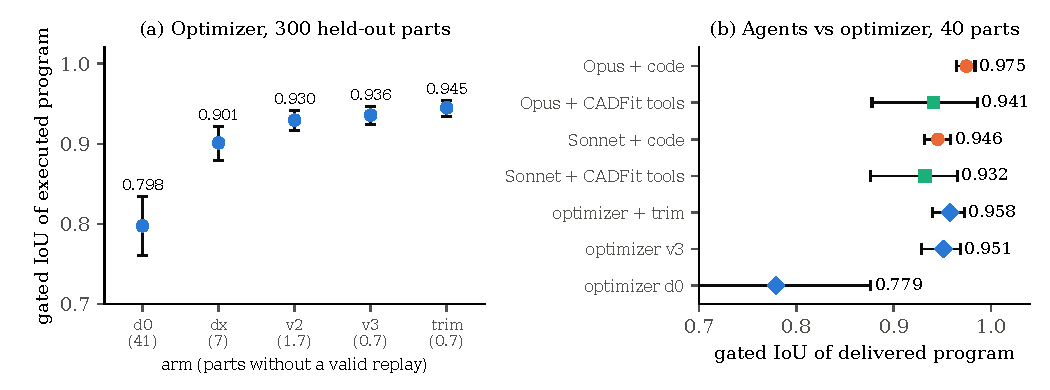
\includegraphics[width=\linewidth]{figures/hero.pdf}
\caption{\textbf{(a)} Search arms on \nFresh{} fresh parts. Light bars score the mesh the search reports; dark bars score the solid built by executing the final program. Error bars: 95\% bootstrap intervals of the mean over parts. Red: unbuilt + OCC-invalid programs; n/m = validity not measured for the best-of control. \textbf{(b)} Six open-weight agents on \nAgentParts{} of those parts, writing CadQuery alone (open) or with CADFit stages as tools (filled); failed episodes score 0. Vertical lines: the strongest pipeline arm on the same parts and two scripted policies over the same tools; the unrestricted one is labelled with its free ground-truth trials.}
\label{fig:hero}
\end{figure}

Our answers, summarised in \cref{fig:hero}:
\begin{enumerate}
\item \textbf{Execution changes the ranking of search extensions} (\cref{sec:search}). The gap between mesh IoU and \iouc{} grows from the base pipeline (\armBaseGap) to beam search (\armBeamGap), almost entirely through programs that do not build. Gains in \iouc{} are measurably smaller than gains in mesh IoU for the rule package and for the full ladder of extensions. We also document measurement defects in the stock objective and judge, including an alpha-wrapped objective, cavity filling and self-intersecting lofts, that change individual scores (\cref{sec:measure}).
\item \textbf{Whole-part section proposals survive execution} (\cref{sec:search}). Adding a mid-plane section extrusion per axis to the candidate pool is the largest observed \iouc{} increment among our extensions (\dSecBeamCadDiff, 95\% interval \dSecBeamCadCI). The gain is concentrated on benchE; over the corrected base pipeline the overall \iouc{} gain is not established.
\item \textbf{Optimizer stages are effective tools for open-weight agents} (\cref{sec:agents}). With the stages as tools, all six models improve over writing CadQuery alone, by \skillsGainMin{} to \skillsGainMax{} \iouc{}, and every Bonferroni-corrected interval excludes zero. The best agent's mean is \mGemmaVsPipeDiff{} relative to the strongest pipeline arm on the same parts (interval \mGemmaVsPipeCI). A scripted policy with the same tools and budget is not shown to be worse than any agent.
\end{enumerate}

The evaluation protocol, the extensions, the agent harness and every script that regenerates our tables are released with the paper.

\section{Related work}
\label{sec:related}

\paragraph{Mesh- and point-cloud-to-CAD.}
Learned methods map geometry to construction sequences: DeepCAD \citep{wu2021deepcad} and Point2Cyl \citep{uy2022point2cyl} predict sketch-and-extrude structure, zone graphs \citep{xu2021zonegraphs} search over extrusion sequences, and CAD-Recode \citep{rukhovich2025cadrecode} decodes point clouds into CadQuery code that is executed for evaluation. CADFit \citep{nehme2026cadfit} optimizes instead: it fits extrusion and revolve candidates to slices of the mesh and composes them greedily to maximize volumetric IoU. Datasets include ABC \citep{koch2019abc}, Fusion 360 Gallery \citep{willis2021fusion360} and DeepCAD; CADBench \citep{doris2026cadbench} unifies them with face-count tiers and metrics for fidelity, executability and compactness. Our contribution is an audit-and-repair study of one optimizer under an executed, validity-gated endpoint, with each repair tested on held-out parts.

\paragraph{Iterative and agentic CAD generation.}
Tool-using language models \citep{yao2023react,schick2023toolformer} and agent--computer interfaces \citep{yang2024sweagent} motivate CAD agents that act, observe and revise. CADReasoner \citep{kabisov2026cadreasoner} trains a model to edit a runnable CadQuery program from the geometric discrepancy of its previous output, and IterCAD \citep{hu2026itercad} trains a multimodal agent against an executable CAD sandbox. CAD-Assistant \citep{mallis2025cadassistant} plans FreeCAD actions with CAD-specific tools, and CADFather \citep{savrasov2026cadfather} coordinates learned and algorithmic proposal tools with a vision-language assistant, executes the proposed programs and keeps the best valid one. CADSmith \citep{barkley2026cadsmith} wraps text-to-CadQuery generation in nested loops that fix execution errors and check geometry programmatically, and RA-CAD \citep{yan2026racad} learns to critique a program after executing it. We use frozen closed models without training, take the tools from one optimizer, and compare two tool packages on a cohort drawn after both were frozen.

\begin{table}[t]
\centering
\small
\caption{Positioning by evaluation design. \emph{Search signal}: what the system optimizes or selects on. \emph{Final replay}: the reported score is computed on the solid built by re-executing the final delivered program. \emph{Zero-inclusive}: failed deliveries enter the fidelity average as zero. \emph{Prospective}: arms and analysis fixed before a cohort drawn for the study. n.r.: not reported in that work.}
\label{tab:related}
\setlength{\tabcolsep}{3.5pt}
\resizebox{\linewidth}{!}{%
\begin{tabular}{@{}llllll@{}}
\toprule
Work & Input & Search signal & Final replay & Zero-inclusive & Prospective \\
\midrule
CADFit & mesh & mesh IoU; kernel validity reported & n.r. & n.r. & n.r. \\
CAD-Recode & point cloud & learned decoder & yes & n.r. & n.r. \\
CADReasoner & renders, points & executed output & yes & n.r. & n.r. \\
CADFather & mesh & executed programs & yes & n.r. & n.r. \\
This work & mesh & mesh IoU (optimizer), executed IoU (agents) & yes & yes & yes \\
\bottomrule
\end{tabular}}
\end{table}

\section{Execution-based evaluation}
\label{sec:protocol}

\paragraph{Executed program.} Every system delivers a CadQuery program \citep{cadquery}. We run it in a fresh sandboxed process with no network access and a 900\,s limit, take its result solid, and check OCC validity of the shape and of every solid it contains. A program that fails to build, builds an invalid solid, exceeds the limit, or is missing is a failed delivery.

\paragraph{Judge.} The executed solid is tessellated and compared with the target, normalized so that its largest extent spans $[-1,1]$. When both meshes are closed and consistently oriented, IoU is computed exactly with manifold booleans \citep{manifold3d}; otherwise it is a seeded Monte-Carlo estimate in which inside-ness of the reconstruction is the generalized winding number \citep{jacobson2013winding}, so a tessellation cracked by float round-off is not judged as a hollow shell. \textbf{Validity-gated IoU} is the IoU of the executed solid if the delivery succeeded and 0 otherwise. Every cohort part stays in every denominator.

\paragraph{Cohorts.} All parts are hard-tier CADBench \citep{doris2026cadbench} solids from two splits, benchA and benchE, drawn by seeded shuffles that exclude every source model already used in any earlier set. Development used separate sets (\cref{app:cohorts}). \textbf{fresh2} (150 + 150 parts) was drawn after development for the optimizer study; \textbf{40 reserved parts} (20 + 20) were drawn from fresh2's manifest before any fresh2 outcome existed and used for the agent study; \textbf{fresh3} (20 + 20) was drawn after the revised tools and their protocol were frozen. The optimizer's outcomes on fresh2's other 260 parts were seen before the agent studies began; fresh3 is the only cohort unseen by every analysis.

\paragraph{Statistics.} All comparisons are paired over parts. Repeated runs or episodes are averaged within part first. Intervals are nominal 95\% bootstrap intervals that resample parts within split \citep{efron1993bootstrap}. Tests are exact two-sided sign tests on per-part differences; a part counts as better or worse when its difference exceeds $\pm0.005$ in the optimizer study and $\pm10^{-9}$ in the agent studies, and as neutral otherwise. Holm correction is applied within each declared family (stated per study).

\paragraph{Preregistration and amendments.} Each study's arms, cohort, primary and secondary comparisons and analysis code were committed before its runs. Changes made after outcomes existed are recorded as dated amendments, reported in the main text with their effect, and listed with every exclusion and rerun in \cref{app:log}.

\begin{figure}[t]
\centering
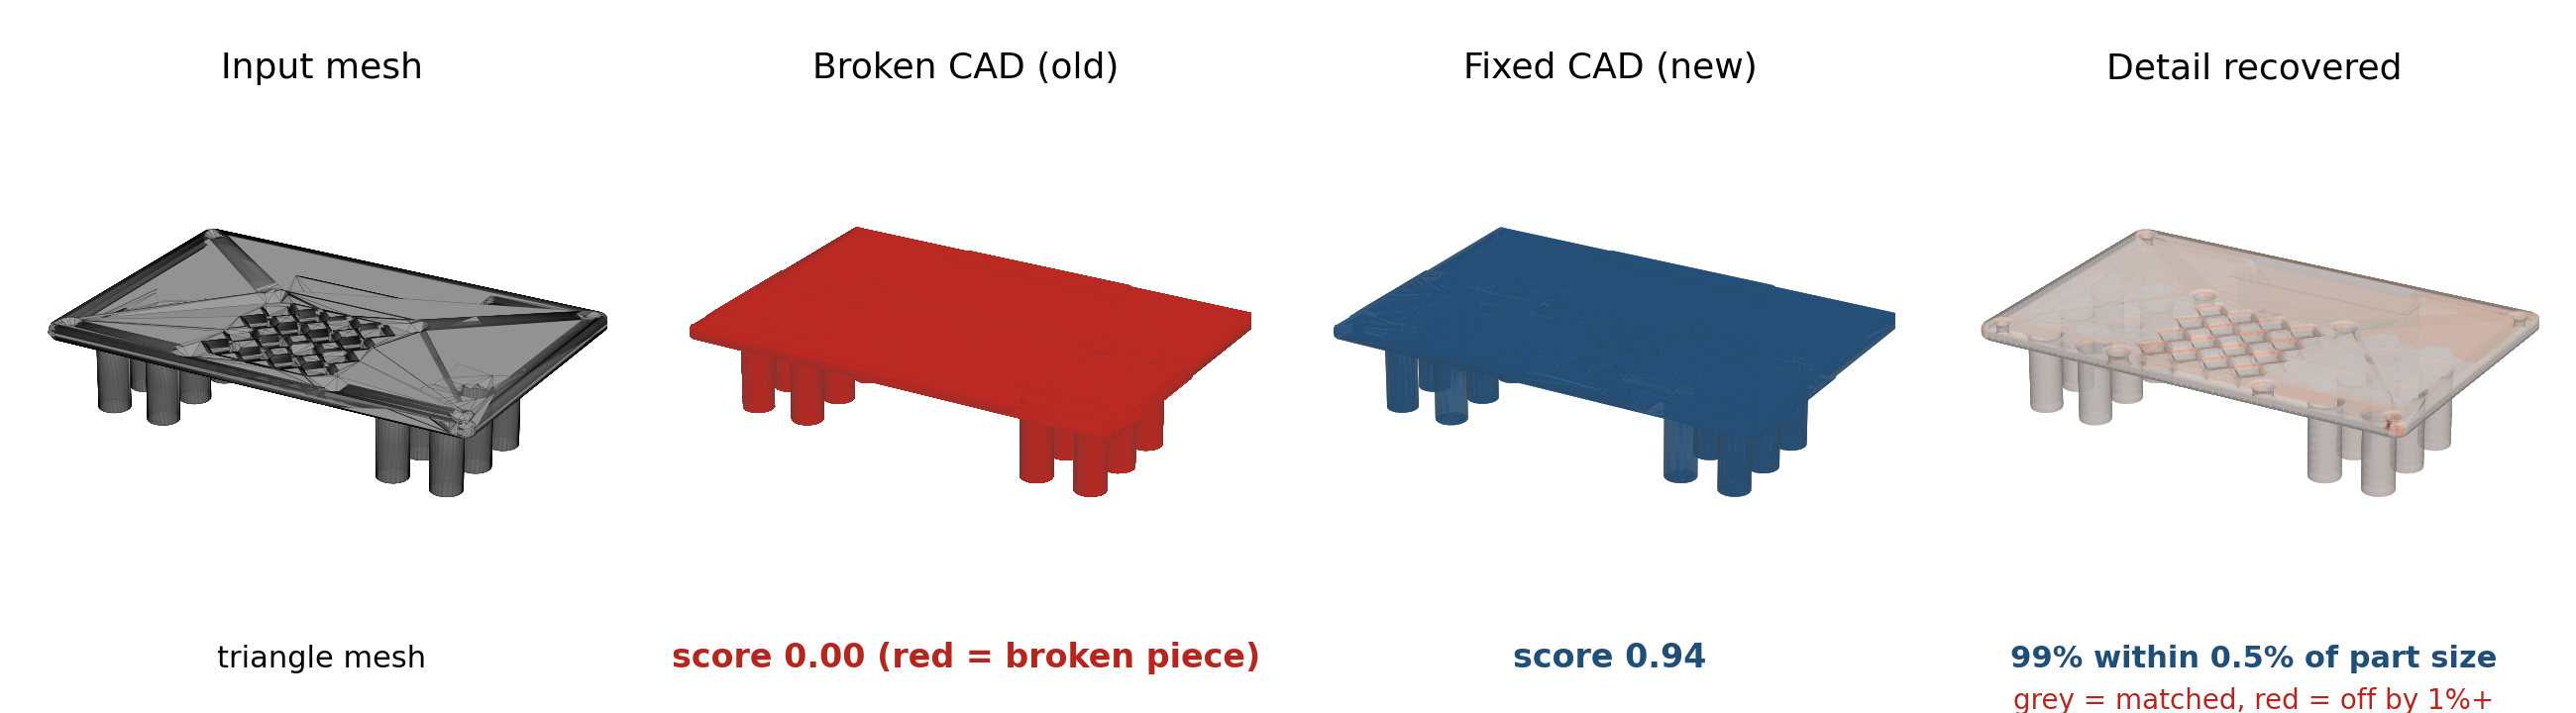
\includegraphics[width=\linewidth]{figures/detail.png}
\caption{A development part (not from any evaluation cohort). Left to right: the input mesh; the program written by the optimizer's search, which stacks 208 overlapping solids of which 34 are OCC-invalid (red) and therefore scores 0; the program delivered by the execution check, a fused rewrite with one valid solid (IoU 0.94, as recorded by the pipeline); the input surface colored by distance to that delivery (grey within 0.5\% of the part size).}
\label{fig:detail}
\end{figure}

\section{Study 1: the optimizer on held-out parts}
\label{sec:optimizer}

\paragraph{Arms.} All arms run frozen source trees on the 300 fresh2 parts. \textbf{d0} is the released CADFit pipeline with two common fixes applied to every arm (a memory bound on mesh decimation with a retry of crashed CadQuery workers, and a seeded surface sampler for the revolve-axis search). \textbf{dx} adds execution-verified delivery: each candidate program is executed and checked, the best valid one is delivered, and an invalid result is fused or repaired (ShapeFix per invalid solid, dropping a solid that stays invalid) before falling back. \textbf{v2} adds geometry fixes to candidate generation and composition; \textbf{v3} adds precise extrusion extents (extent sweep, finer steps along thin directions, ends snapped to cap planes with the unsnapped candidate kept); \textbf{trim} adds a silhouette-trimmed variant (the best valid program intersected with prisms over the target's three axis silhouettes) as one more candidate for the execution check. d0 and dx run once; v2, v3 and trim run with three seeds, averaged within part. The primary contrast, dx~$-$~d0, is analysed alone; the secondary family (Holm over four tests) is v2~$-$~dx, v3~$-$~v2, trim~$-$~v3 and trim against a section-only reference (one executed mid-plane section extrusion per axis, best of three).

\begin{table}[t]
\centering
\small
\caption{Study 1, 300 held-out fresh2 parts (after the recovery amendment). Gated IoU of the executed program; v2, v3 and trim are averaged over three seeds within part and their valid counts are given per seed (min--max). Minutes: mean and median successful-attempt wall time per part (299 measured per run; three parts usually shared a node; retries excluded). Failure classes per run are in \cref{tab:failures}.}
\label{tab:optimizer}
\setlength{\tabcolsep}{4.5pt}
\resizebox{\linewidth}{!}{%
\begin{tabular}{@{}lcccccc@{}}
\toprule
Arm & Gated IoU & benchA & benchE & Valid / 300 & Mean min & Median min \\
\midrule
d0 (released) & \hDZero & \hDZeroA & \hDZeroE & \hDZeroValid & \hMinDZero & \hMedDZero \\
dx (+ exec.-verified delivery) & \hDX & \hDXA & \hDXE & \hDXValid & \hMinDX & \hMedDX \\
v2 (+ geometry fixes) & \hVTwo & \hVTwoA & \hVTwoE & \hValidVTwoLo--\hValidVTwoHi & \hMinVTwo & \hMedVTwo \\
v3 (+ precise extents) & \hVThree & \hVThreeA & \hVThreeE & \hValidVThreeLo--\hValidVThreeHi & \hMinVThree & \hMedVThree \\
trim (+ silhouette trim) & \hTrim & \hTrimA & \hTrimE & \hValidTrimLo--\hValidTrimHi & \multicolumn{2}{c}{partial (see text)} \\
section-only reference & \hSection & & & & & \\
\midrule
\multicolumn{7}{@{}l}{\emph{Contrasts} (difference, 95\% interval, parts better/worse/neutral at $\pm0.005$, $p$)} \\
dx $-$ d0 (primary) & \multicolumn{6}{l}{\hDXvsDZero{} \hDXvsDZeroCI, \hDXvsDZeroWL/\hDXvsDZeroNeutral, $p$ \hDXvsDZeroP} \\
v2 $-$ dx & \multicolumn{6}{l}{\hVTwovsDX{} \hVTwovsDXCI, \hVTwovsDXWL/\hVTwovsDXNeutral, Holm$_3$ $p$ \hVTwovsDXP} \\
v3 $-$ v2 & \multicolumn{6}{l}{\hVThreevsVTwo{} \hVThreevsVTwoCI, \hVThreevsVTwoWL/\hVThreevsVTwoNeutral, Holm$_3$ $p$ \hVThreevsVTwoP} \\
trim $-$ v3 & \multicolumn{6}{l}{\hTrimvsVThree{} \hTrimvsVThreeCI, \hTrimvsVThreeWL/\hTrimvsVThreeNeutral, Holm$_3$ $p$ \hTrimvsVThreeP} \\
trim $-$ section-only & \multicolumn{6}{l}{\hTrimvsSection} \\
\bottomrule
\end{tabular}}
\end{table}

\paragraph{Execution-verified delivery.} The released pipeline obtains a valid replay on \fDZeroValid{} of 300 parts. Of the 41 failures, \fDZeroBuiltInvalid{} programs build an OCC-invalid solid, \fDZeroBuildError{} raise a build error, \fDZeroMissing{} produced no program, and \fDZeroResource{} exceed the replay limits (time or memory); the last class says nothing about the geometry and is scored 0 under the protocol. Delivering the best program that actually builds valid raises gated IoU from \hDZero{} to \hDX{} (\cref{tab:optimizer}), a primary contrast of \hDXvsDZero{} \hDXvsDZeroCI. The gain comes from validity: on parts where both arms deliver a valid program the mean difference is \hDXvsDZeroBothValid.

\paragraph{Later stages.} Each later stage adds a smaller, significant increment: \hVTwovsDX{} for the geometry fixes, \hVThreevsVTwo{} for precise extents, and \hTrimvsVThree{} for the trim (better/worse \hTrimvsVThreeWL). These adjusted $p$-values are Holm over the three available tests and are provisional until the fourth (trim against the section-only reference) is computed. The trim arm also re-runs the fuse/repair pass before trimming. Over all 300 parts and per seed, that pass changes gated IoU by \hRepassLo{} to \hRepassHi{} (the negative value is one seed-0 replay that timed out inside the trim run and is kept as a frozen 0), and the trim itself adds \hTrimProperLo{} to \hTrimProperHi.

\paragraph{Recovery amendment.} The first scoring pass stored replay failures that were not evaluations: on one node the sandbox could not be set up (dx: 299 parts), and one v2 seed hit the 900\,s limit on 222 parts that the other seeds replayed. After those outcomes were visible we adopted, for all eight runs, a rule giving every setup or resource-limit failure one terminal recovery evaluation with the same judge and limit; programs were not regenerated. It affected \hRecoveredTotal{} records. d0's ten resource failures failed again and stay 0; dx and the v2 seed recovered. On the original records the primary contrast is \hPreDXvsDZero{} (dx valid on \hPreDXValid{} part) and the three-seed v2 mean is \hPreMeanVTwox{} instead of \hMeanVTwox. Both analyses are in \cref{app:recovery}; we report the recovered one as the measurement and label it as amended.

\paragraph{Runtime.} Execution checking costs time: mean minutes per part rise from \hMinDZero{} (d0) to \hMinDX{} (dx) and \hMinVThree{} (v3); medians from \hMedDZero{} to \hMedVThree. These are successful-attempt wall times on CPU nodes that usually ran three parts at once; retried attempts are excluded, so they are not total compute. The trim run's timer starts after its initial replay and repair, so its full latency is not measured.

\paragraph{Pending outputs.} The section-only reference (\hSection), an independent re-judging of every delivered program with a different seed and four times the samples (\hRejudge), and surface agreement on the fused boundary (\hSurface) are still being computed; no claim here depends on them.

\section{Study 2: frontier agents under the same judge}
\label{sec:agents}

\paragraph{Harness.} An agent receives the target only through tools and edits a model step by step. After every change, the harness assembles the CadQuery program, executes and checks it as in \cref{sec:protocol}, and reports build status, validity and executed IoU; the delivered answer is the best executed valid program, or, if no check of a valid program finished within the episode, the current program unverified (it is still re-judged offline like every other delivery). The \textbf{code} toolset is \texttt{describe\_target} (size, volume, flat-face directions and offsets), \texttt{section} (exact cross-sections of target and model), \texttt{evaluate}, \texttt{add\_code}, \texttt{remove\_step}, \texttt{list\_steps} and \texttt{finish}: it gives target inspection and execution feedback, so it is not an unaided language-model baseline. The \textbf{CADFit} toolset adds the optimizer's stages: direction detection, sketch extraction on a plane with line/arc fitting, extrusion and revolve fitting, section extrusion, and candidate management. Each episode has 40 tool calls and 30 minutes.

\paragraph{Models and runs.} Claude Opus~5.5 (\texttt{claude-opus-5-5}) and Sonnet~5.5 (\texttt{claude-sonnet-5-5}) run through the Anthropic Messages API with adaptive thinking at effort high, at most 32k output tokens per turn, the full conversation history, and no server-side fallback to another model. Each model runs three independent episodes per part and toolset on the 40 reserved parts; every delivered program is re-judged offline by the same replay and judge as the optimizer. These comparisons were specified after the optimizer study and are exploratory; intervals are nominal.

\begin{figure}[t]
\centering
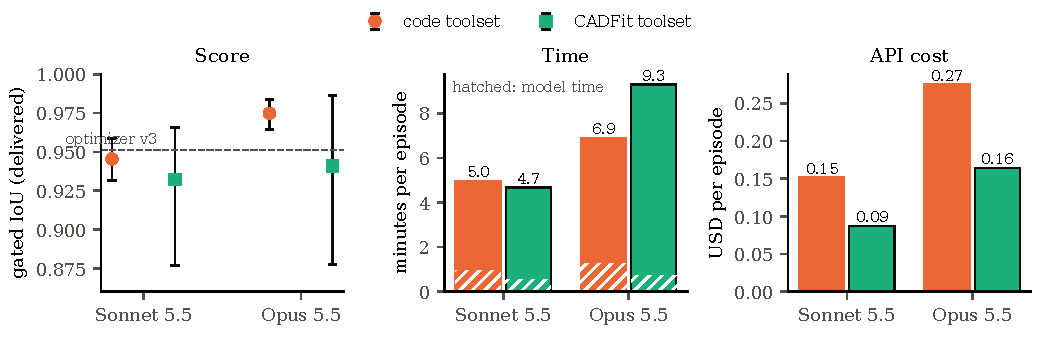
\includegraphics[width=\linewidth]{figures/closed.pdf}
\caption{Study 2, 40 reserved fresh2 parts, three episodes per part and condition. Left: gated IoU of the delivered program (mean over parts of the per-part mean; 95\% interval); dashed: the optimizer's v3 on the same parts. Middle: mean minutes per episode, hatched part waiting on the model. Right: mean API cost per episode. Runtime and cost are means without intervals.}
\label{fig:closed}
\end{figure}

\begin{table}[t]
\centering
\small
\caption{Study 2 against the optimizer on the same 40 parts (gated IoU, 95\% interval). Valid: delivered programs that build valid / episodes; no-output episodes ended at the deadline with nothing delivered. Differences are paired over parts (better/worse); exploratory.}
\label{tab:agents}
\setlength{\tabcolsep}{4pt}
\resizebox{\linewidth}{!}{%
\begin{tabular}{@{}lcccccc@{}}
\toprule
 & Gated IoU & 95\% interval & Valid & No output & Mean min & USD / episode \\
\midrule
Opus + code & \cOpusCode & \cOpusCodeCI & \cOpusCodeValid & \cOpusCodeNoOut & \cOpusCodeMin & \cOpusCodeCost \\
Opus + CADFit tools & \cOpusSkills & \cOpusSkillsCI & \cOpusSkillsValid & \cOpusSkillsNoOut & \cOpusSkillsMin & \cOpusSkillsCost \\
Sonnet + code & \cSonnetCode & \cSonnetCodeCI & \cSonnetCodeValid & \cSonnetCodeNoOut & \cSonnetCodeMin & \cSonnetCodeCost \\
Sonnet + CADFit tools & \cSonnetSkills & \cSonnetSkillsCI & \cSonnetSkillsValid & \cSonnetSkillsNoOut & \cSonnetSkillsMin & \cSonnetSkillsCost \\
\midrule
optimizer d0 / dx & \cPipeDZero{} / \cPipeDX & & & & & \\
optimizer v3 / + trim & \cPipeVThree{} / \cPipeTrim & \cPipeVThreeCI{} / \cPipeTrimCI & & & & \\
\midrule
Opus code $-$ v3 & \multicolumn{6}{l}{\cOpusCodeVsVThree{} \cOpusCodeVsVThreeCI, \cOpusCodeVsVThreeWL} \\
Opus code $-$ trim & \multicolumn{6}{l}{\cOpusCodeVsTrim{} \cOpusCodeVsTrimCI, \cOpusCodeVsTrimWL} \\
CADFit tools $-$ code & \multicolumn{6}{l}{Opus \cOpusSkillsVsCode{} \cOpusSkillsVsCodeCI; Sonnet \cSonnetSkillsVsCode{} \cSonnetSkillsVsCodeCI} \\
\bottomrule
\end{tabular}}
\end{table}

\paragraph{Results.} Opus with the code toolset scores \cOpusCode{} with \cOpusCodeValid{} valid deliveries (\cref{fig:closed}, \cref{tab:agents}). On the same parts the optimizer's v3 scores \cPipeVThree; the paired difference \cOpusCodeVsVThree{} \cOpusCodeVsVThreeCI{} excludes zero, while the difference from the optimizer with trim, \cOpusCodeVsTrim{} \cOpusCodeVsTrimCI, does not, so superiority over the full optimizer package is not established. Opus exceeds Sonnet with the code toolset by \cOpusVsSonnetCode{} \cOpusVsSonnetCodeCI, better on \cOpusVsSonnetCodeWL{} parts.

\paragraph{The optimizer's stages as tools.} With the CADFit toolset, the mean differences from code are \cOpusSkillsVsCode{} \cOpusSkillsVsCodeCI{} for Opus and \cSonnetSkillsVsCode{} \cSonnetSkillsVsCodeCI{} for Sonnet. All \cDeliveredValid{} programs the agents delivered are valid; the CADFit arms also contain \cOpusSkillsNoOut{} (Opus) and \cSonnetSkillsNoOut{} (Sonnet) episodes that reached the deadline with nothing delivered, on three parts, and these score zero. Offline validity is not the same as in-episode verification: \cValidUnverified{} valid deliveries had not completed an executed check within their episode.

\paragraph{Where the time goes.} Tool execution, not the model, dominates episodes: \texttt{add\_code}, whose cost is the executed check after every change, takes \cAddCodeShareLo--\cAddCodeShareHi\% of tool time in the code arms, and single calls of the CADFit stages reached \cMaxCall\,s. Mean minutes per episode are \cOpusCodeMin{} (Opus, code) to \cOpusSkillsMin{} (Opus, CADFit tools); the optimizer's v3 takes \hMinFortyVThree{} minutes per part on these parts, on different hardware and without API cost.

\section{Study 3: removing the tools' overhead}
\label{sec:tools}

\paragraph{Profiling.} On development parts only, we timed every stage inside the tool calls of a scripted policy that uses the CADFit tools. Sketch extraction spent \eExtractFitShare\% of its time (\eProfileParts{} development parts) fitting lines and arcs to every profile on the plane; a function-level profile of one development part attributed most of that to two routines: duplicate-point removal by an all-pairs loop, and a greedy segmenter that refits the whole run with an SVD each time it extends by one point. Revolve fitting rotated points one at a time in Python, and every executed check reloaded and rebuilt the target.

\paragraph{The revised package (tools v3).} Four changes are exact rewrites, each checked against the old code on development inputs: KD-tree duplicate removal (identical output on \eDedup{} randomized cases), the segment error from running sums with the old SVD fit deciding whenever a value lies within $10^{-6}$ (relative) of a threshold it is compared with (identical fitted output on \eFit{} sketches from \eFitParts{} development parts and 9 planes; fitting time \eFitOld\,s $\to$ \eFitNew\,s together with the first change), vectorized rotation (bit-identical on \eRotation{} cases), and loading the target once per process in the judge (\eJudge{} identical); the checks are recorded in \texttt{results/tools/equivalence.json}. One change alters behaviour: each executed check gets at most 120\,s. A step whose check does not finish stays in the model unchecked and is never delivered while a checked valid program exists. The study tests this package as a whole; it does not separate the rewrites from the cap.

\paragraph{Design.} The protocol fixed, before any run and before the cohort was drawn: tools \{v2, v3\} $\times$ toolset \{code, CADFit\} $\times$ \{Opus, Sonnet\} on the 40 fresh3 parts, three episodes each (960 episodes), same budget and settings as Study 2, each version running from its own frozen tree, delivered programs re-judged offline. The primary comparison is Opus with CADFit tools, v3 $-$ v2; the Opus family (primary, CADFit tools v3 $-$ code v3, code v3 $-$ v2) is Holm-corrected over three sign tests; the same comparisons for Sonnet are reported uncorrected. Runtime summaries were prespecified; timing contrasts and their tests are descriptive. Episodes lost to API credit exhaustion, rate limits, a faulty node and one client timeout crash were set aside and rerun before any analysis (\cref{app:log}).

\begin{figure}[t]
\centering
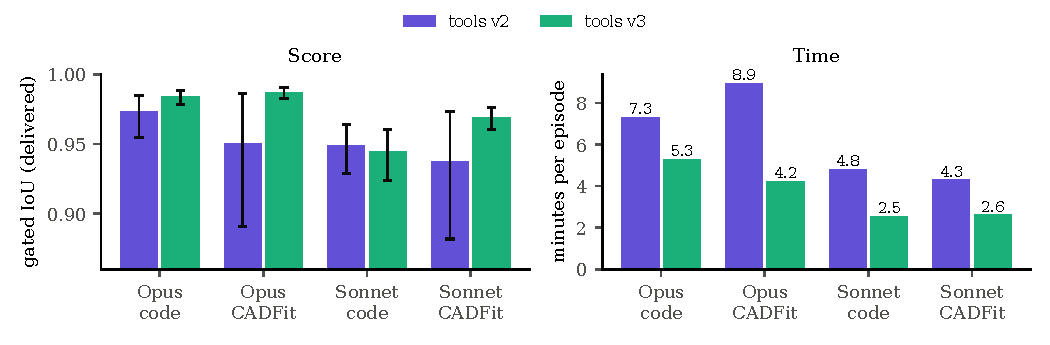
\includegraphics[width=\linewidth]{figures/tools_v3.pdf}
\caption{Study 3, 40 fresh3 parts, three episodes per part and condition. Left: gated IoU of the delivered program (95\% interval). Right: mean minutes per episode (means without intervals).}
\label{fig:tools}
\end{figure}

\begin{table}[t]
\centering
\small
\caption{Study 3 comparisons (gated IoU, paired over parts; better/worse at $\pm10^{-9}$; sign test $p$; Holm over the three Opus tests). Below: mean minutes per part, v3 $-$ v2 (descriptive), with parts faster.}
\label{tab:tools}
\setlength{\tabcolsep}{4pt}
\begin{tabular}{@{}llccc@{}}
\toprule
Comparison & & Difference \& 95\% interval & Better/worse & $p$ (Holm) \\
\midrule
Opus & CADFit v3 $-$ v2 (primary) & \tOpusSkillsVersion{} \tOpusSkillsVersionCI & \tOpusSkillsVersionWL & \tOpusSkillsVersionP{} (\tOpusSkillsVersionHolm) \\
Opus & CADFit v3 $-$ code v3 & \tOpusSkillsVsCode{} \tOpusSkillsVsCodeCI & \tOpusSkillsVsCodeWL & \tOpusSkillsVsCodeP{} (\tOpusSkillsVsCodeHolm) \\
Opus & code v3 $-$ v2 & \tOpusCodeVersion{} \tOpusCodeVersionCI & \tOpusCodeVersionWL & \tOpusCodeVersionP{} (\tOpusCodeVersionHolm) \\
Sonnet & CADFit v3 $-$ v2 & \tSonnetSkillsVersion{} \tSonnetSkillsVersionCI & \tSonnetSkillsVersionWL & \tSonnetSkillsVersionP \\
Sonnet & CADFit v3 $-$ code v3 & \tSonnetSkillsVsCode{} \tSonnetSkillsVsCodeCI & \tSonnetSkillsVsCodeWL & \tSonnetSkillsVsCodeP \\
Sonnet & code v3 $-$ v2 & \tSonnetCodeVersion{} \tSonnetCodeVersionCI & \tSonnetCodeVersionWL & \tSonnetCodeVersionP \\
\midrule
\multicolumn{2}{@{}l}{Minutes, v3 $-$ v2} & Opus CADFit \tTimeOpusSkills{} \tTimeOpusSkillsCI & faster on \tTimeOpusSkillsFaster/40 & \tTimeOpusSkillsP \\
 & & Opus code \tTimeOpusCode{} \tTimeOpusCodeCI & \tTimeOpusCodeFaster/40 & \tTimeOpusCodeP \\
 & & Sonnet CADFit \tTimeSonnetSkills{} \tTimeSonnetSkillsCI & \tTimeSonnetSkillsFaster/40 & \tTimeSonnetSkillsP \\
 & & Sonnet code \tTimeSonnetCode{} \tTimeSonnetCodeCI & \tTimeSonnetCodeFaster/40 & \tTimeSonnetCodeP \\
\bottomrule
\end{tabular}
\end{table}

\paragraph{Results.} The primary comparison is positive, \tOpusSkillsVersion{} \tOpusSkillsVersionCI, but its declared sign test does not establish an improvement ($p=\tOpusSkillsVersionP$, Holm \tOpusSkillsVersionHolm); we do not read it as evidence of no effect either (\cref{tab:tools}). With tools v3, Opus delivers a valid program in all \tOpusSkillsVThreeValid{} episodes with the CADFit tools (v2: \tOpusSkillsVTwoValid, with \tOpusSkillsVTwoNoOut{} no-output and \tOpusSkillsVTwoInvalid{} invalid), and those tools beat plain code by \tOpusSkillsVsCode{} \tOpusSkillsVsCodeCI, better on \tOpusSkillsVsCodeWL{} parts, Holm $p=\tOpusSkillsVsCodeHolm$: a small but consistent advantage, the reverse of the sign seen with tools v2 in Study 2. For Sonnet the same contrast is \tSonnetSkillsVsCode{} \tSonnetSkillsVsCodeCI{} (uncorrected $p=\tSonnetSkillsVsCodeP$). The best cell, Opus with CADFit tools v3, scores \tOpusSkillsVThree{} \tOpusSkillsVThreeCI. Across all 960 episodes, \tDeliveredValid{} delivered programs are valid offline, of which \tValidUnverified{} had not completed an in-episode check.

\paragraph{Time.} Mean minutes per part with the CADFit tools fall from \tOpusSkillsVTwoMin{} to \tOpusSkillsVThreeMin{} for Opus, faster on \tTimeOpusSkillsFaster{} of 40 parts, and from \tSonnetSkillsVTwoMin{} to \tSonnetSkillsVThreeMin{} for Sonnet. In the other cells the mean also falls, but the per-part sign tests are not significant, and the means are dominated by a few parts that used to run long. Opus with code v2 reproduces Study 2 on this new cohort (\tOpusCodeVTwo{} here, \cOpusCode{} there).

\section{Discussion and limitations}
\label{sec:discussion}

\paragraph{What changes when the program is executed.} The largest held-out improvement to the optimizer came from no new geometry at all: delivering the program that actually builds valid recovered most of what the search had found. Under the same execution-based judge, a frontier model with inspection, plain code and execution feedback reached the optimizer's level on reserved held-out parts, at a few minutes and cents per part. The optimizer's stages first looked useless as agent tools; profiling located the cost in redundant computation, and with a revised package (exact rewrites plus a per-check time cap) those stages gave the strongest agent a small, consistent edge over plain code. Measuring tools by their cost as well as their output therefore changed the conclusion about them; which part of the package matters was not isolated.

\paragraph{Limitations.} (i) The optimizer study's measurement was amended after outcomes were visible (one terminal recovery evaluation for setup and resource-limit replay failures); the original analysis is reported beside it, and it changes the dx and v2 values substantially. (ii) The agent studies use 40 parts per cohort with three episodes each, so many intervals are several hundredths of IoU wide, and the Study 2 comparisons are exploratory. (iii) One benchmark: hard-tier CADBench parts from two splits. (iv) The endpoint is volumetric IoU; surface agreement and an independent re-judging are pending. (v) The code toolset includes target inspection and execution feedback, so it measures an agent in this harness, not a language model alone. (vi) Closed-model results are tied to specific model versions, settings (32k tokens per turn, full history) and an API; the tools-v3 package bundles exact rewrites with a behavioural check cap, and its output-equivalence was checked on development inputs only. (vii) Infrastructure failures (faulty nodes, API limits) required reruns, listed in \cref{app:log}.


\section*{Reproducibility statement}
Result values in the tables and text are macros generated from committed result files by \texttt{bench/paper\_numbers.py}, apart from a few counts quoted from the protocols' execution logs (e.g.\ the recovery classes), and every figure is drawn by a committed script; configuration constants, cohort dates and the counts of the development example in \cref{fig:detail} come from the protocols, the code and the pipeline's records. The protocols, with their dated amendments and execution logs, the frozen source trees of every arm, the cohort definitions (seeded draws excluding earlier model indices), the scoring and analysis code, and the per-part and per-episode records will be released with the paper. Closed-model episodes require an Anthropic API key; their raw records are included, so the analyses can be re-run without the API.


\bibliography{references}
\bibliographystyle{iclr2027_conference}

\appendix
\section{Agent harness details}
\label{app:harness}
\paragraph{Sandbox.} Agent-written code and the replay of every final program run in a sandbox with no network and writes confined to the episode folder: bubblewrap where available; otherwise an unprivileged user namespace in which every mount is remounted read-only and verified (the sandbox refuses to run if any mount stays writable), temporary directories are replaced by empty file systems, the episode folder is bound back read-write, and all capabilities are dropped with no-new-privileges set.

\paragraph{Context.} The last six tool results are kept in full; older results, older assistant text and older code arguments are truncated to 300 characters in what is sent back. Tool results are capped at 8{,}000 characters while remaining valid JSON. On a context-length error the kept window halves.

\paragraph{Models.}
\begin{center}
\scriptsize
\resizebox{\linewidth}{!}{% generated by bench/paper_tables.py -- do not edit
\begin{tabular}{@{}llp{6.6cm}@{}}
\toprule
model & temperature & request extras and vLLM parsers \\
\midrule
Gemma-4-31B (\texttt{google/gemma-4-31B-it}) & 1.0 & \texttt{\{"top\_p": 0.95, "top\_k": 64, "chat\_template\_kwargs": \{"enable\_thinking": true\}\}}; \texttt{--reasoning-parser gemma4 --tool-call-parser gemma4} \\
Qwen3.6-35B-A3B (\texttt{Qwen/Qwen3.6-35B-A3B-FP8}) & 1.0 & \texttt{\{"top\_p": 0.95, "top\_k": 20, "min\_p": 0.0, "presence\_penalty": 0.0, "chat\_template\_kwargs": \{"enable\_thinking": true\}\}}; \texttt{--reasoning-parser qwen3 --tool-call-parser qwen3\_coder --language-model-only} \\
gpt-oss-120b (\texttt{openai/gpt-oss-120b}) & 1.0 & \texttt{\{"top\_p": 1.0\}}; \texttt{--reasoning-parser openai\_gptoss --tool-call-parser openai} \\
Devstral-S-2-24B (\texttt{mistralai/Devstral-Small-2-24B-Instruct-2512}) & 0.15 & \texttt{\{\}}; \texttt{--tool-call-parser mistral --tokenizer-mode mistral --config-format mistral --load-format mistral} \\
gpt-oss-20b (\texttt{openai/gpt-oss-20b}) & 1.0 & \texttt{\{"top\_p": 1.0\}}; \texttt{--reasoning-parser openai\_gptoss --tool-call-parser openai} \\
Qwen3.8-27B (\texttt{Qwen/Qwen3.8-27B-FP8}) & 1.0 & \texttt{\{"top\_p": 0.95, "top\_k": 20, "min\_p": 0.0, "presence\_penalty": 0.0, "chat\_template\_kwargs": \{"enable\_thinking": true\}\}}; \texttt{--reasoning-parser qwen3 --tool-call-parser qwen3\_xml --language-model-only} \\
\bottomrule
\end{tabular}
}
\end{center}

\paragraph{Prompts.} The three system prompts differ only in the tool paragraph and the strategy phrase.
% generated by bench/paper_tables.py -- do not edit
\paragraph{System prompt, \texttt{code} toolset.}
{\scriptsize\begin{verbatim}
You are a CAD engineer. Your job: build a solid CAD model that matches a target 3D part as
    closely as possible, measured by volumetric IoU (intersection over union) against the
    target.

You cannot see the target. You learn about it only through tools:
- describe_target: size, volume, and the flat faces (directions and plane positions).
- section: exact cross-section polygons of the target (and of your model) in any
    axis-aligned plane.
- add_code: append a solid built by your CadQuery code to the model as a union ('add') or a
    difference ('cut').
- evaluate: current IoU and where material is missing or extra.
- remove_step, list_steps, finish.

Coordinates: everything is in the normalized frame (the target is centered and scaled so
    its largest extent spans [-1, 1]). Your CadQuery code (cq and math are imported) must
    assign the final solid to `result`, e.g.
    result = cq.Workplane('XY').box(1.2, 0.8, 0.1).translate((0, 0, 0.35))
    result = cq.Workplane('XY', origin=(0, 0, -0.2)).circle(0.3).extrude(0.4)
    result =
    cq.Workplane('XZ').polyline([(0,0),(0.5,0),(0.5,0.2),(0,0.2)]).close().revolve(360,
    (0,0,0), (0,1,0))

Good strategy: describe the target, read sections to get exact profile shapes, build the
    main body first, then add features and cut holes/pockets, checking evaluate after
    changes and removing steps that lower IoU. The best model seen at any point is kept, so
    experimenting is safe. Work efficiently: you have a limited number of tool calls. Call
    finish when you cannot improve further.
\end{verbatim}}
\paragraph{System prompt, \texttt{codesec} toolset.}
{\scriptsize\begin{verbatim}
You are a CAD engineer. Your job: build a solid CAD model that matches a target 3D part as
    closely as possible, measured by volumetric IoU (intersection over union) against the
    target.

You cannot see the target. You learn about it only through tools:
- describe_target: size, volume, and the flat faces (directions and plane positions).
- section: exact cross-section polygons of the target (and of your model) in any
    axis-aligned plane.
- section_extrude: a CADFit stage that extrudes the target's whole cross-section at a plane
    through the full extent of the part. Each solid it makes becomes a scored candidate:
    list_candidates / show_candidate show them; precision near 1 means the candidate lies
    inside the target.
- add_candidate / add_code: append a solid to the model as a union ('add') or a difference
    ('cut').
- evaluate: current IoU and where material is missing or extra.
- remove_step, list_steps, finish.

Coordinates: everything is in the normalized frame (the target is centered and scaled so
    its largest extent spans [-1, 1]). Your CadQuery code (cq and math are imported) must
    assign the final solid to `result`, e.g.
    result = cq.Workplane('XY').box(1.2, 0.8, 0.1).translate((0, 0, 0.35))
    result = cq.Workplane('XY', origin=(0, 0, -0.2)).circle(0.3).extrude(0.4)
    result =
    cq.Workplane('XZ').polyline([(0,0),(0.5,0),(0.5,0.2),(0,0.2)]).close().revolve(360,
    (0,0,0), (0,1,0))

Good strategy: describe the target, read sections to get exact profile shapes and extrude
    whole cross-sections, build the main body first, then add features and cut
    holes/pockets, checking evaluate after changes and removing steps that lower IoU. The
    best model seen at any point is kept, so experimenting is safe. Work efficiently: you
    have a limited number of tool calls. Call finish when you cannot improve further.
\end{verbatim}}
\paragraph{System prompt, \texttt{skills} toolset.}
{\scriptsize\begin{verbatim}
You are a CAD engineer. Your job: build a solid CAD model that matches a target 3D part as
    closely as possible, measured by volumetric IoU (intersection over union) against the
    target.

You cannot see the target. You learn about it only through tools:
- describe_target: size, volume, and the flat faces (directions and plane positions).
- section: exact cross-section polygons of the target (and of your model) in any
    axis-aligned plane.
- CADFit skills, the stages of a CAD reconstruction pipeline, which you run yourself:
    detect_directions (likely extrusion directions), extract_sketch (slice the target at a
    plane into sketch profiles fitted with lines and arcs), fit_extrude / fit_revolve (turn
    a sketch into extrusion / revolve solids that match the target), section_extrude
    (extrude a whole cross-section through the part). Each solid they make becomes a scored
    candidate: list_candidates / show_candidate show them; precision near 1 means the
    candidate lies inside the target.
- add_candidate / add_code: append a solid to the model as a union ('add') or a difference
    ('cut').
- evaluate: current IoU and where material is missing or extra.
- remove_step, list_steps, finish.

Coordinates: everything is in the normalized frame (the target is centered and scaled so
    its largest extent spans [-1, 1]). Your CadQuery code (cq and math are imported) must
    assign the final solid to `result`, e.g.
    result = cq.Workplane('XY').box(1.2, 0.8, 0.1).translate((0, 0, 0.35))
    result = cq.Workplane('XY', origin=(0, 0, -0.2)).circle(0.3).extrude(0.4)
    result =
    cq.Workplane('XZ').polyline([(0,0),(0.5,0),(0.5,0.2),(0,0.2)]).close().revolve(360,
    (0,0,0), (0,1,0))

Good strategy: describe the target, extract sketches on its main planes and fit them into
    candidates, build the main body first, then add features and cut holes/pockets,
    checking evaluate after changes and removing steps that lower IoU. The best model seen
    at any point is kept, so experimenting is safe. Work efficiently: you have a limited
    number of tool calls. Call finish when you cannot improve further.
\end{verbatim}}


\section{Tool use}
\label{app:tools}
Tool calls per episode in the skills toolset, over the \nAgentParts{} episodes of each model (\texttt{results/tool\_usage.json}).
\begin{center}
\scriptsize
\resizebox{\linewidth}{!}{% generated by bench/paper_tables.py -- do not edit
\begin{tabular}{@{}lcccccccccccc@{}}
\toprule
model & calls & \rotatebox{70}{\texttt{extract\_sketch}} & \rotatebox{70}{\texttt{fit\_extrude}} & \rotatebox{70}{\texttt{fit\_revolve}} & \rotatebox{70}{\texttt{section\_extrude}} & \rotatebox{70}{\texttt{detect\_directions}} & \rotatebox{70}{\texttt{section}} & \rotatebox{70}{\texttt{add\_candidate}} & \rotatebox{70}{\texttt{add\_code}} & \rotatebox{70}{\texttt{evaluate}} & \rotatebox{70}{\texttt{remove\_step}} & errors \\
\midrule
Gemma-4-31B & 27.9 & 3.1 & 2.7 & 0.1 & 1.1 & 0.4 & 6.0 & 2.9 & 3.5 & 1.9 & 2.6 & 17/559 \\
Qwen3.6-35B-A3B & 37.2 & 4.9 & 2.2 & 0.0 & 1.6 & 1.0 & 12.3 & 2.5 & 3.4 & 2.2 & 2.5 & 47/744 \\
gpt-oss-120b & 38.2 & 4.8 & 3.6 & 0.1 & 1.6 & 1.0 & 6.6 & 4.0 & 3.6 & 3.0 & 3.4 & 22/764 \\
Devstral-S-2-24B & 37.2 & 3.8 & 6.8 & 0.3 & 1.2 & 0.9 & 2.7 & 7.2 & 3.4 & 4.1 & 3.9 & 12/745 \\
gpt-oss-20b & 25.1 & 2.1 & 1.8 & 0.1 & 1.6 & 0.9 & 6.2 & 2.6 & 2.2 & 2.6 & 1.2 & 44/503 \\
Qwen3.8-27B & 22.2 & 1.8 & 1.6 & 0.0 & 0.3 & 1.0 & 7.9 & 1.3 & 3.1 & 1.3 & 1.8 & 27/445 \\
\bottomrule
\end{tabular}
}
\end{center}

\section{Qwen3.8 token-limit failures and a post-hoc sensitivity run}
\label{app:qwen}
The harness sends ``Your reply hit the token limit before you called a tool. Think briefly, then call a tool now.'' only when a reply ends because it reached the 16{,}384-token limit; after two consecutive nudges without a tool call the episode stops. In all \qwenTraceN{} Qwen3.8 code episodes that stopped this way, the last nudge was the token-limit message, and the final reply was \qwenTraceMinK--\qwenTraceMaxK{} thousand characters of reasoning with no content (\texttt{results/qwen38\_traces.json}). After seeing these outcomes we reran Qwen3.8 on the same parts with 32{,}768 tokens per turn. It scored \qwenPosthocSkills{} with skills and \qwenPosthocCode{} with code (versus \mQwenEightSkills{} and \mQwenEightCode{} at 16{,}384). Because this run was decided after seeing results, it is excluded from \cref{tab:agents}; most of its episodes ended at the 30-minute limit instead.

\section{Refining pipeline output with an LLM agent}
\label{app:refine}
In an earlier study, Qwen3.8-27B (INT4) refined arm C's output on the \refN{} fresh parts whose C mesh IoU was below 0.90 (gate fixed before running), with access to C's candidate pool, 40 calls and 20 minutes, in two runs. Mean mesh IoU: pipeline \refPipe; agent \refAgentOne{} and \refAgentTwo{} (wins--losses against the pipeline at a $\pm 0.01$ threshold: \refAgentOneWL{} and \refAgentTwoWL); a no-op agent that only re-exports the pipeline model \refNoop; an equal-time scripted search over the same pool \refSearch{} (\refSearchWL). The mean gain comes from a few parts and does not repeat consistently. Per-part records were not retained, so no intervals or executed-program scores are available for this study.

\section{Per-part results}
\label{app:perpart}
{\scriptsize
% generated by bench/paper_tables.py -- do not edit
\begin{longtable}{@{}llcccccccc@{}}
\toprule
part & split & A mesh & A CAD & B mesh & B CAD & C mesh & C CAD & D mesh & D CAD \\
\midrule\endhead
00038011 & A & 0.844 & 0.844 & 0.939 & 0.937 & 0.940 & 0.940 & 0.940 & 0.940 \\
00046097 & A & 0.896 & 0.915 & 0.939 & 0.940 & 0.942 & 0.943 & 0.942 & 0.943 \\
00053172 & E & 0.994 & 0.994 & 0.994 & 0.994 & 0.994 & 0.994 & 0.998 & 0.998 \\
00090768 & A & 0.962 & 0.962 & 0.971 & 0.971 & 0.999 & 0.967 & 0.999 & 0.002 \\
00095369 & A & 0.882 & 0.882 & 0.893 & 0.893 & 0.893 & 0.893 & 0.948 & 0.948 \\
00101419 & A & 0.965 & 0.965 & 0.978 & 0.978 & 0.978 & 0.978 & 1.000 & 1.000 \\
00140273 & E & 0.884 & 0.884 & 0.884 & 0.884 & 0.884 & 0.884 & 0.894 & 0.894 \\
00153120 & E & 0.771 & 0.771 & 0.857 & 0.857 & 0.857 & 0.857 & 0.996 & 0.996 \\
00154184 & E & 0.000 & --$^\dagger$ & 0.980 & 0.981 & 0.984 & 0.984 & 0.984 & 0.984 \\
00161800 & A & 0.985 & 0.985 & 0.985 & 0.985 & 0.985 & 0.985 & 0.985 & 0.985 \\
00181393 & A & 0.863 & 0.863 & 0.863 & 0.863 & 0.863 & 0.863 & 0.863 & 0.863 \\
00208290 & E & 0.989 & 0.989 & 0.989 & 0.989 & 0.989 & 0.989 & 0.992 & 0.992 \\
00214289 & A & 0.997 & 0.997 & 0.989 & 0.989 & 0.989 & 0.989 & 0.989 & 0.989 \\
00232213 & E & 0.837 & 0.837 & 0.869 & 0.000$^\dagger$ & 0.861 & 0.873$^*$ & 0.869 & 0.000$^\dagger$ \\
00246395 & E & 0.959 & 0.959 & 0.959 & 0.959 & 0.959 & 0.959 & 0.997 & 0.997 \\
00247424 & E & 0.000 & --$^\dagger$ & 0.000 & --$^\dagger$ & 0.000 & --$^\dagger$ & 0.000 & --$^\dagger$ \\
00249450 & E & 0.926 & 0.926 & 0.960 & 0.960 & 0.960 & 0.960 & 0.995 & 0.995 \\
00256926 & E & 0.814 & 0.814 & 0.892 & 0.892 & 0.899 & 0.902 & 1.000 & 1.000 \\
00266468 & E & 0.723 & 0.724 & 0.746 & 0.746 & 0.749 & 0.746 & 1.000 & 1.000 \\
00273535 & E & 0.912 & 0.912 & 0.995 & 0.995 & 0.995 & 0.995 & 1.000 & 1.000 \\
00299355 & E & 0.975 & 0.976 & 0.975 & 0.976 & 0.975 & 0.976 & 0.990 & 0.990 \\
00305871 & E & 0.960 & 0.960 & 0.961 & 0.961 & 0.961 & 0.961 & 1.000 & 1.000 \\
00312587 & E & 0.973 & 0.973 & 0.975 & 0.974 & 0.975 & 0.974 & 1.000 & 1.000 \\
00317970 & E & 0.182 & 0.182 & 0.733 & 0.743 & 0.746 & 0.747 & 0.993 & 0.993 \\
00354176 & A & 0.896 & 0.896 & 0.903 & 0.904 & 0.903 & 0.904 & 0.903 & 0.904 \\
00365747 & A & 0.848 & 0.848 & 0.880 & 0.000$^\dagger$ & 0.888 & 0.000$^\dagger$ & 0.961 & 0.956$^*$ \\
00382121 & A & 0.920 & 0.920 & 0.933 & 0.933 & 0.936 & 0.934 & 0.936 & 0.936 \\
00492401 & A & 0.975 & 0.986 & 0.986 & 0.986 & 0.987 & 0.988 & 0.987 & 0.987 \\
00528181 & A & 0.860 & 0.876 & 0.915 & 0.916$^*$ & 0.882 & 0.882 & 0.960 & 0.958 \\
00562677 & A & 0.867 & 0.867 & 0.889 & 0.889 & 0.889 & 0.889 & 0.889 & 0.889 \\
00589302 & A & 0.921 & 0.921 & 0.966 & 0.966 & 0.969 & 0.937$^*$ & 0.949 & 0.949 \\
00630878 & A & 0.848 & 0.849 & 0.942 & 0.944 & 0.944 & 0.944 & 0.944 & 0.944 \\
00634093 & A & 0.931 & 0.931 & 0.941 & 0.942 & 0.946 & 0.946 & 0.946 & 0.946 \\
00642725 & A & 0.908 & 0.908 & 0.931 & 0.000$^\dagger$ & 0.930 & 0.000$^\dagger$ & 0.936 & 0.000$^\dagger$ \\
00657371 & E & 0.901 & 0.902 & 0.901 & 0.902 & 0.902 & 0.903 & 0.987 & 0.987 \\
00678171 & E & 0.935 & 0.935 & 0.945 & 0.945 & 0.945 & 0.945 & 0.949 & 0.949 \\
00700032 & A & 0.855 & 0.855 & 0.885 & 0.881 & 0.886 & 0.886 & 0.955 & 0.955 \\
00709520 & A & 0.888 & 0.889 & 0.888 & 0.889 & 0.888 & 0.889 & 0.888 & 0.889 \\
00729452 & A & 0.051 & 0.053 & 0.280 & 0.281 & 0.280 & 0.281 & 0.280 & 0.281 \\
00730725 & E & 0.018 & 0.018 & 0.018 & 0.018 & 0.018 & 0.018 & 0.949 & 0.949 \\
00771160 & E & 0.890 & 0.900 & 0.974 & 0.974 & 0.985 & 0.982$^*$ & 0.985 & 0.982$^*$ \\
00771600 & E & 0.919 & 0.919 & 0.919 & 0.919 & 0.920 & 0.920 & 0.999 & 0.999 \\
00780711 & E & 0.911 & 0.911 & 0.973 & 0.973 & 0.983 & 0.983 & 0.983 & 0.983 \\
00791454 & E & 0.970 & 0.970 & 0.970 & 0.970 & 0.970 & 0.970 & 0.990 & 0.990 \\
00795057 & E & 0.949 & 0.949 & 0.969 & 0.969 & 0.980 & 0.980 & 0.997 & 0.997 \\
00814797 & E & 0.933 & 0.933 & 0.970 & 0.970 & 0.970 & 0.970 & 0.999 & 0.999 \\
00834538 & A & 0.920 & 0.920 & 0.948 & 0.948 & 0.954 & 0.949 & 0.968 & 0.968 \\
00846352 & A & 0.859 & 0.859 & 0.859 & 0.859 & 0.867 & 0.867 & 0.867 & 0.867 \\
00862084 & A & 0.593 & 0.593 & 0.553 & 0.557 & 0.639 & 0.648 & 0.999 & 0.999 \\
00862085 & E & 0.422 & 0.422 & 0.475 & 0.475 & 0.475 & 0.475 & 0.999 & 0.999 \\
00862953 & E & 0.796 & 0.796 & 0.802 & 0.804 & 0.802 & 0.804 & 0.980 & 0.980 \\
00883892 & E & 0.792 & 0.792 & 0.905 & 0.906 & 0.913 & 0.000$^\dagger$ & 0.900 & 0.900 \\
00892314 & A & 0.916 & 0.916 & 0.933 & 0.940$^*$ & 0.935 & 0.000$^\dagger$ & 0.959 & 0.959 \\
00904252 & A & 0.977 & 0.977 & 0.977 & 0.977 & 0.977 & 0.977 & 0.977 & 0.977 \\
00941601 & A & 0.923 & 0.923 & 0.943 & 0.943 & 0.947 & 0.947 & 0.949 & 0.949 \\
00953658 & E & 0.973 & 0.973 & 0.976 & 0.976 & 0.978 & 0.978 & 0.982 & 0.982 \\
00966049 & A & 0.815 & 0.815 & 0.945 & 0.818 & 0.945 & 0.818 & 0.950 & 0.821 \\
00966713 & E & 0.994 & 0.994 & 0.994 & 0.994 & 0.994 & 0.994 & 0.998 & 0.998 \\
00983172 & A & 0.877 & 0.877 & 0.993 & 0.985 & 0.993 & 0.000$^\dagger$ & 0.984 & 0.984 \\
00992810 & A & 0.879 & 0.879 & 0.995 & 0.995 & 0.995 & 0.995 & 0.997 & 0.997 \\
\bottomrule
\end{longtable}

}
$^\dagger$ program does not build; $^*$ builds but fails OpenCascade validity.

\begin{table}[h]
\centering
\caption{Per-part \iouc{} of the agent study (failures 0).}
\resizebox{\linewidth}{!}{% generated by bench/paper_tables.py -- do not edit
\begin{tabular}{@{}lcccccccccccccc@{}}
\toprule
part & \multicolumn{2}{c}{Gemma-4-31B} & \multicolumn{2}{c}{Qwen3.6-35B-A3B} & \multicolumn{2}{c}{gpt-oss-120b} & \multicolumn{2}{c}{Devstral-S-2-24B} & \multicolumn{2}{c}{gpt-oss-20b} & \multicolumn{2}{c}{Qwen3.8-27B} & policy & pipe D \\
 & code & skills & code & skills & code & skills & code & skills & code & skills & code & skills & & \\
\midrule
00046097 & 0.389 & 0.832 & 0.000 & 0.739 & 0.702 & 0.770 & 0.274 & 0.765 & 0.844 & 0.739 & 0.000 & 0.785 & 0.776 & 0.943 \\
00095369 & 0.955 & 0.951 & 0.945 & 0.872 & 0.866 & 0.953 & 0.086 & 0.838 & 0.873 & 0.872 & 0.945 & 0.986 & 0.899 & 0.948 \\
00140273 & 0.251 & 0.894 & 0.439 & 0.884 & 0.446 & 0.894 & 0.308 & 0.894 & 0.245 & 0.647 & 0.000 & 0.000 & 0.894 & 0.894 \\
00153120 & 0.976 & 0.996 & 0.410 & 0.996 & 0.976 & 0.996 & 0.227 & 0.971 & 0.579 & 0.996 & 0.749 & 0.996 & 0.996 & 0.996 \\
00154184 & 0.230 & 0.967 & 0.168 & 0.936 & 0.268 & 0.218 & 0.211 & 0.218 & 0.151 & 0.195 & 0.000 & 0.971 & 0.810 & 0.984 \\
00232213 & 0.121 & 0.279 & 0.399 & 0.304 & 0.228 & 0.276 & 0.126 & 0.458 & 0.243 & 0.000 & 0.000 & 0.000 & 0.403 & 0.000 \\
00249450 & 0.980 & 0.979 & 0.980 & 0.995 & 0.942 & 0.995 & 0.327 & 0.881 & 0.651 & 0.995 & 0.978 & 0.980 & 0.995 & 0.995 \\
00354176 & 0.021 & 0.929 & 0.221 & 0.929 & 0.313 & 0.930 & 0.221 & 0.929 & 0.281 & 0.929 & 0.566 & 0.929 & 0.000 & 0.904 \\
00492401 & 0.647 & 0.932 & 0.231 & 0.934 & 0.602 & 0.847 & 0.343 & 0.883 & 0.292 & 0.848 & 0.000 & 0.910 & 0.871 & 0.987 \\
00528181 & 0.221 & 0.889 & 0.472 & 0.765 & 0.196 & 0.889 & 0.252 & 0.706 & 0.164 & 0.765 & 0.000 & 0.732 & 0.784 & 0.958 \\
00589302 & 0.747 & 0.948 & 0.950 & 0.974 & 0.950 & 0.948 & 0.652 & 0.669 & 0.950 & 0.948 & 0.000 & 0.824 & 0.948 & 0.949 \\
00630878 & 0.252 & 0.951 & 0.000 & 0.658 & 0.255 & 0.747 & 0.181 & 0.676 & 0.265 & 0.615 & 0.000 & 0.835 & 0.746 & 0.944 \\
00700032 & 0.961 & 0.962 & 0.608 & 0.962 & 0.960 & 0.962 & 0.326 & 0.962 & 0.614 & 0.962 & 0.975 & 0.963 & 0.962 & 0.955 \\
00771600 & 0.944 & 0.999 & 0.618 & 0.999 & 0.618 & 0.621 & 0.713 & 0.919 & 0.000 & 0.999 & 0.000 & 0.985 & 0.999 & 0.999 \\
00834538 & 0.816 & 0.969 & 0.319 & 0.968 & 0.816 & 0.968 & 0.183 & 0.966 & 0.816 & 0.968 & 0.813 & 0.968 & 0.968 & 0.968 \\
00862084 & 0.933 & 0.999 & 0.157 & 0.999 & 0.489 & 0.905 & 0.161 & 0.798 & 0.124 & 0.993 & 0.926 & 0.975 & 0.999 & 0.999 \\
00883892 & 0.668 & 0.773 & 0.590 & 0.669 & 0.676 & 0.789 & 0.590 & 0.572 & 0.590 & 0.793 & 0.169 & 0.000 & 0.793 & 0.900 \\
00941601 & 0.289 & 0.898 & 0.332 & 0.740 & 0.030 & 0.873 & 0.489 & 0.731 & 0.338 & 0.000 & 0.000 & 0.916 & 0.740 & 0.949 \\
00953658 & 0.628 & 0.929 & 0.622 & 0.929 & 0.623 & 0.929 & 0.415 & 0.893 & 0.415 & 0.622 & 0.000 & 0.844 & 0.929 & 0.982 \\
00966049 & 0.830 & 0.764 & 0.836 & 0.823 & 0.176 & 0.735 & 0.011 & 0.790 & 0.000 & 0.763 & 0.018 & 0.000 & 0.679 & 0.821 \\
\bottomrule
\end{tabular}
}
\end{table}


\end{document}
